% degree=[master]                             % 必选,学位类型
% language=[chinese|english],                 % 可选(默认:chinese),论文的主要语言
% review=[true|false]					      % 可选,盲审,默认为false
% bibstyle=[gb7714-2015|gb7714-2015ay|ieee],  % 可选(默认:gb7714-2015),参考文献样式
\documentclass[degree=master, language=chinese, review=false, oneside, AutoFakeBold]{shmtuthesis}

% 所有其它可能用到的包都统一放到shmtuthesis.sty中,可以根据自己的实际添加或者删除。
\usepackage{shmtuthesis}

% 定义图片文件目录与扩展名
\graphicspath{{figures/}}
\DeclareGraphicsExtensions{.pdf, .eps, .png, .jpg, .jpeg}

% 导入参考文献数据库
\addbibresource{thesis.bib}

% 论文信息,必须
\title{船岸连接}
\entitle{Ship Shore Connection}
\degreecategory{专业学位}
\author{辛浩东}
\enauthor{John Xin}
\studentid{202030210206}
\supervisor{耿攀}
\ensupervisor{Pan Geng}
\major{能源动力}
\enmajor{Electrical Engineering and Automation}
\finisheddate{二〇二一年二月}

\begin{document}
	
	% 无编号内容:论文封面、授权页
	\maketitle
	\makeDeclareOriginality
	\makeDeclareAuthorization
	
	% 使用罗马数字对前言编号
	\frontmatter
	
	% 摘要
	\begin{abstract}
	论文摘要应简短明了,摘要论文的基本信息,体现科研工作的核心思想。内容包括:课题研究的目的;研究内容;研究方法;完成的工作;获得的主要结论;结论的意义。应突出论文的创造性成果和新的见解。
	
	论文摘要还用作编辑《上海海事大学学位论文摘要汇编集》。为了便于文献检索,应注明论文的关键词。关键词应是从论文中选取出来用以表示论文主题内容信息的单词或术语。
	
	\keywords{上海海事大学,忠信笃敬,XeTeX/LaTeX 模版} 
	
	\zhlipsum[3-6]
\end{abstract}

\begin{enabstract}
	The abstract of the paper should be brief and clear. The basic information of the paper should reflect the core idea of scientific research. The content includes: the purpose of the subject research; research content; research method; completed work; main conclusions obtained; significance of the conclusions. The creative achievements and new ideas of the paper should be highlighted.
	
	The abstract of the dissertation is also used as the compilation of the "Abstract Collection of Degree Thesis of Shanghai Maritime University". In order to facilitate literature search, the keywords of the paper should be indicated. Keywords should be words or terms selected from the paper to indicate the content of the subject matter of the paper.
	
	\lipsum[3-6]

	\enkeywords{SHMTU, Faithful and respectful, XeTeX/LaTeX template}	
\end{enabstract}

	
	% 目录、插图目录、表格目录、算法目录
	\tableofcontents
	\listoffigures
	\listoftables
	\listofalgorithms
	
	% 使用阿拉伯数字对正文编号
	\mainmatter
	
	%我的论文正文
	\chapter{绪论}

\section{课题背景及意义}
绿色能源已成为当今世界能源发展的主要趋势。未来人类可能会面对全球能源危机,发展绿色能源是能源发展惟一的出路。
各国政府纷纷制定了本国的绿色能源发展计划。在港口码头领域,绿色能源,清洁能源正发挥着越来越重要的作用。

船舶停靠码头时,装卸货物电气设备所需电力主要是从船舶电力系统来获取。船舶靠岸期间,用电是由船上的辅机组提供,
辅机发电会消耗化石燃料,主要是重油或者柴油。发电机组工作过程中,化石燃料的使用会排放诸如氮氧化合物,硫氧化合物,
和粉尘等一些污染物,会对港口空气质量造成一定的影响,同时发电机组会产生较大的噪声,影响港口附近人员的工作和
生活。

为了建立绿色港口,清洁港口,减少污染物的排放,船舶在停靠港口时,可以停止使用用柴油发电机组发电,
改用岸上电力系统提供所需电力。中国是世界上最大的航运国家,2020年,全球前20大集装箱港口中国仍占近半数,前10
大集装箱港口中有7个来自中国,中国港口货物吞吐量连年增长。根据国际海事组织(IMO)研究数据表明,2020年,全球
航运业需要4亿吨燃料,排放14亿吨$CO_{2}$,约占全球$CO_{2}$总排放量的$6\%$。保守的估计,我国每年靠港船舶
消耗的燃料油约为$70$万吨,船舶辅机发电的碳排量占港口总碳排量的40\%\~{}70\%\cite{SP1}。

岸电在美国西海岸已是强制性要求,在我国和一些亚洲国家尚在发展之中。我国交通部颁布的《船舶与港口污染防治专项行动实施方案》
(2015-2020年)对促进岸电发展发挥了巨大作用,截至2020年我国$90\%$的公务船舶、港作船舶靠泊时使用了岸电,
$50\%$的客滚、集装箱和邮轮专业化码头具有向船舶提供岸电的能力。港口应用岸电后,船舶靠港时污染物的排放
明显减少,港口环境得到了改善。应用船岸连接技术,对于港口地区的环境保护有重大的意义,
如果船舶岸电技术得到大力发展,所有靠港船舶都由岸电提供电力,那么既可以降低$30\%$的燃油成本\cite{SP2}和节省部分的维护成本,
也能够帮助港口实现IMO减排目标,为国家绿色可持续发展助力。

国家十四五规划,对碳排放,空气污染物的排放量作出了约束性的规定,推广使用岸电技术是保护港口环境,减排防污的一
大重要举措,对建设生态文明友好型的港口具有重大意义。表\ref{tab:岸电替代效益}中数据为中国沿海港口使用可再生能
源替代辅机发电的污染物和碳排放量对比,船舶靠港使用岸电后,微尘等颗粒物的排放减少了78\%,空气污染物$SO_{x}$、
$NO_{x}$的每\si{kW.h}排放量分别减少了74\%和80.1\%。结果表明,船舶靠港使用岸电的做法在节能和温室气体排放方面帮助
不大,但可以有效减少空气污染物的排放,在港口环境保护中的作用明显。

\begin{table}[!htp]
	\centering
	\caption[中国岸电替代辅机发电的减排表现]{中国岸电替代辅机发电的减排表现\cite{SP3}}
	\label{tab:岸电替代效益}
	\resizebox{\textwidth}{!}{
	\begin{tabular}{c}
		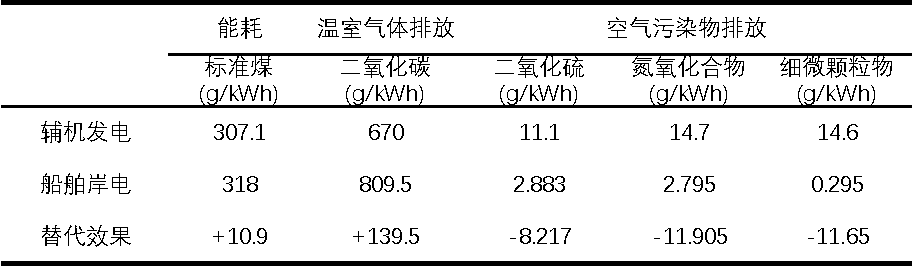
\includegraphics{chapter1/岸电替代效益.pdf} 
	\end{tabular}
	}
\end{table}

电气化,自动化,智能化是全球大趋势,工业过程、城市交通、供热和制冷在未来将由从$CO_{2}$零排放的绿色可再生能源获
得的电力来供电。到 2050年,全球发电容量预计将达到当前发电容量的两倍或三倍,岸电是我国在交通领域实现电气化的重要部分。

\begin{figure}[!htp]
	\centering
	\includegraphics[width=0.87\textwidth]{chapter1/ABB Marine Zero emission port call Infographic.pdf}
	\caption{一种零污染零排放港口示意图}
	\label{fig:一种零污染零排放港口示意图}
\end{figure}

船舶靠港停用辅机改用岸电是港口码头实现防污减排的首选方案,这在全球范围内取得了一定的共识。如图\ref{fig:一种零污染零排放港口示意图}所示,船舶在港口甚至可以实现零污染和零排放。
其次,船舶辅机的发电效率并不是很高,改用岸电后,接入电网计价方便,具有良好的经济替代效益。
最后,发展岸电技术,提高港口自动化率,是中国制造的内在要求。未来,伴随着一带一路的发展,沿线国家的港口势必
会迎来更多的中国货船,推广中国岸电的技术,制定中国岸电技术标准显得十分必要。
中国在成为科技强国的路上,必须大力发展先进技术,在港口领域,我们要大力发展电气化,自动化和智能化的港口,
具体到电气化,则需要大力推广船舶岸电技术,推动船岸连接系统的发展与完善。

\section{船岸连接系统研究现状}
船岸连接技术解决的是港口污染和碳排放超标的问题,受这些问题的影响对该技术研究早在上世纪70年代就开始起步,
发展至今,该技术已经逐步发展完善与成熟,船岸连接系统的相关技术标准也正在趋于完善。
国内外都对船岸连接系统进行了研究与设计,由于国外起步较早,技术成熟且应用广泛,形成了一定的技术标准。
国内起步发展相对较晚,不过近年来随着绿色发展观念的深入人心,在国家的大力倡导下,中国岸电技术发展势头迅猛,
然而国内范围的船岸连接系统许多仍处在试验阶段,发展和推广应用的工作依然任重而道远\cite{SP4}。

\subsection{国外应用状况}
1989年瑞典哥德堡港率先应用船岸连接技术,由于当时的技术限制哥德堡港采用了低压(400V)岸电系统,
船岸连接技术的应用明显改善了港口环境状况。哥德堡港于2000年安装了ABB公司开发的一套高压岸电系统,这也使得哥德堡港成为了世界上
第一个应用高压岸电系统的港口。该系统的电压为6.6kV,容量为1250\si{kV.A},岸电的应用使得停泊船舶的污染物排放量减少了94\%-97\%
\cite{SP4},防治港口污染的作用显著。

2001年,美国朱诺港使用港口岸电向五艘改装的豪华游轮供电,标志着岸电技术在豪华游轮码头的首次应用。岸电系统的成功应用使其
在欧洲和美国引起了广泛的关注。2004年,美国洛杉矶港与中国集装箱船舶公司共同建造的7.5\si{MW}高压岸电系统建成投入使用\cite{SP5},
并计划于2014年在所有集装箱码头安装船舶岸电设施,这是岸电系统在集装箱码头的首次应用。

2009年,美国长滩港首次将岸电系统应用在石油码头,为大型油船提供港口岸电。2012年后,在纽约布鲁克林邮轮码头、安特卫普港集装箱码头、
吕贝克港等也安装了岸电系统。此外,国外诸如东京港、奥克兰港、纽约港、旧金山港等主要港口也正在计划或建设岸电基础设施\cite{SP6}。

\begin{figure}[!htp]
	\centering
	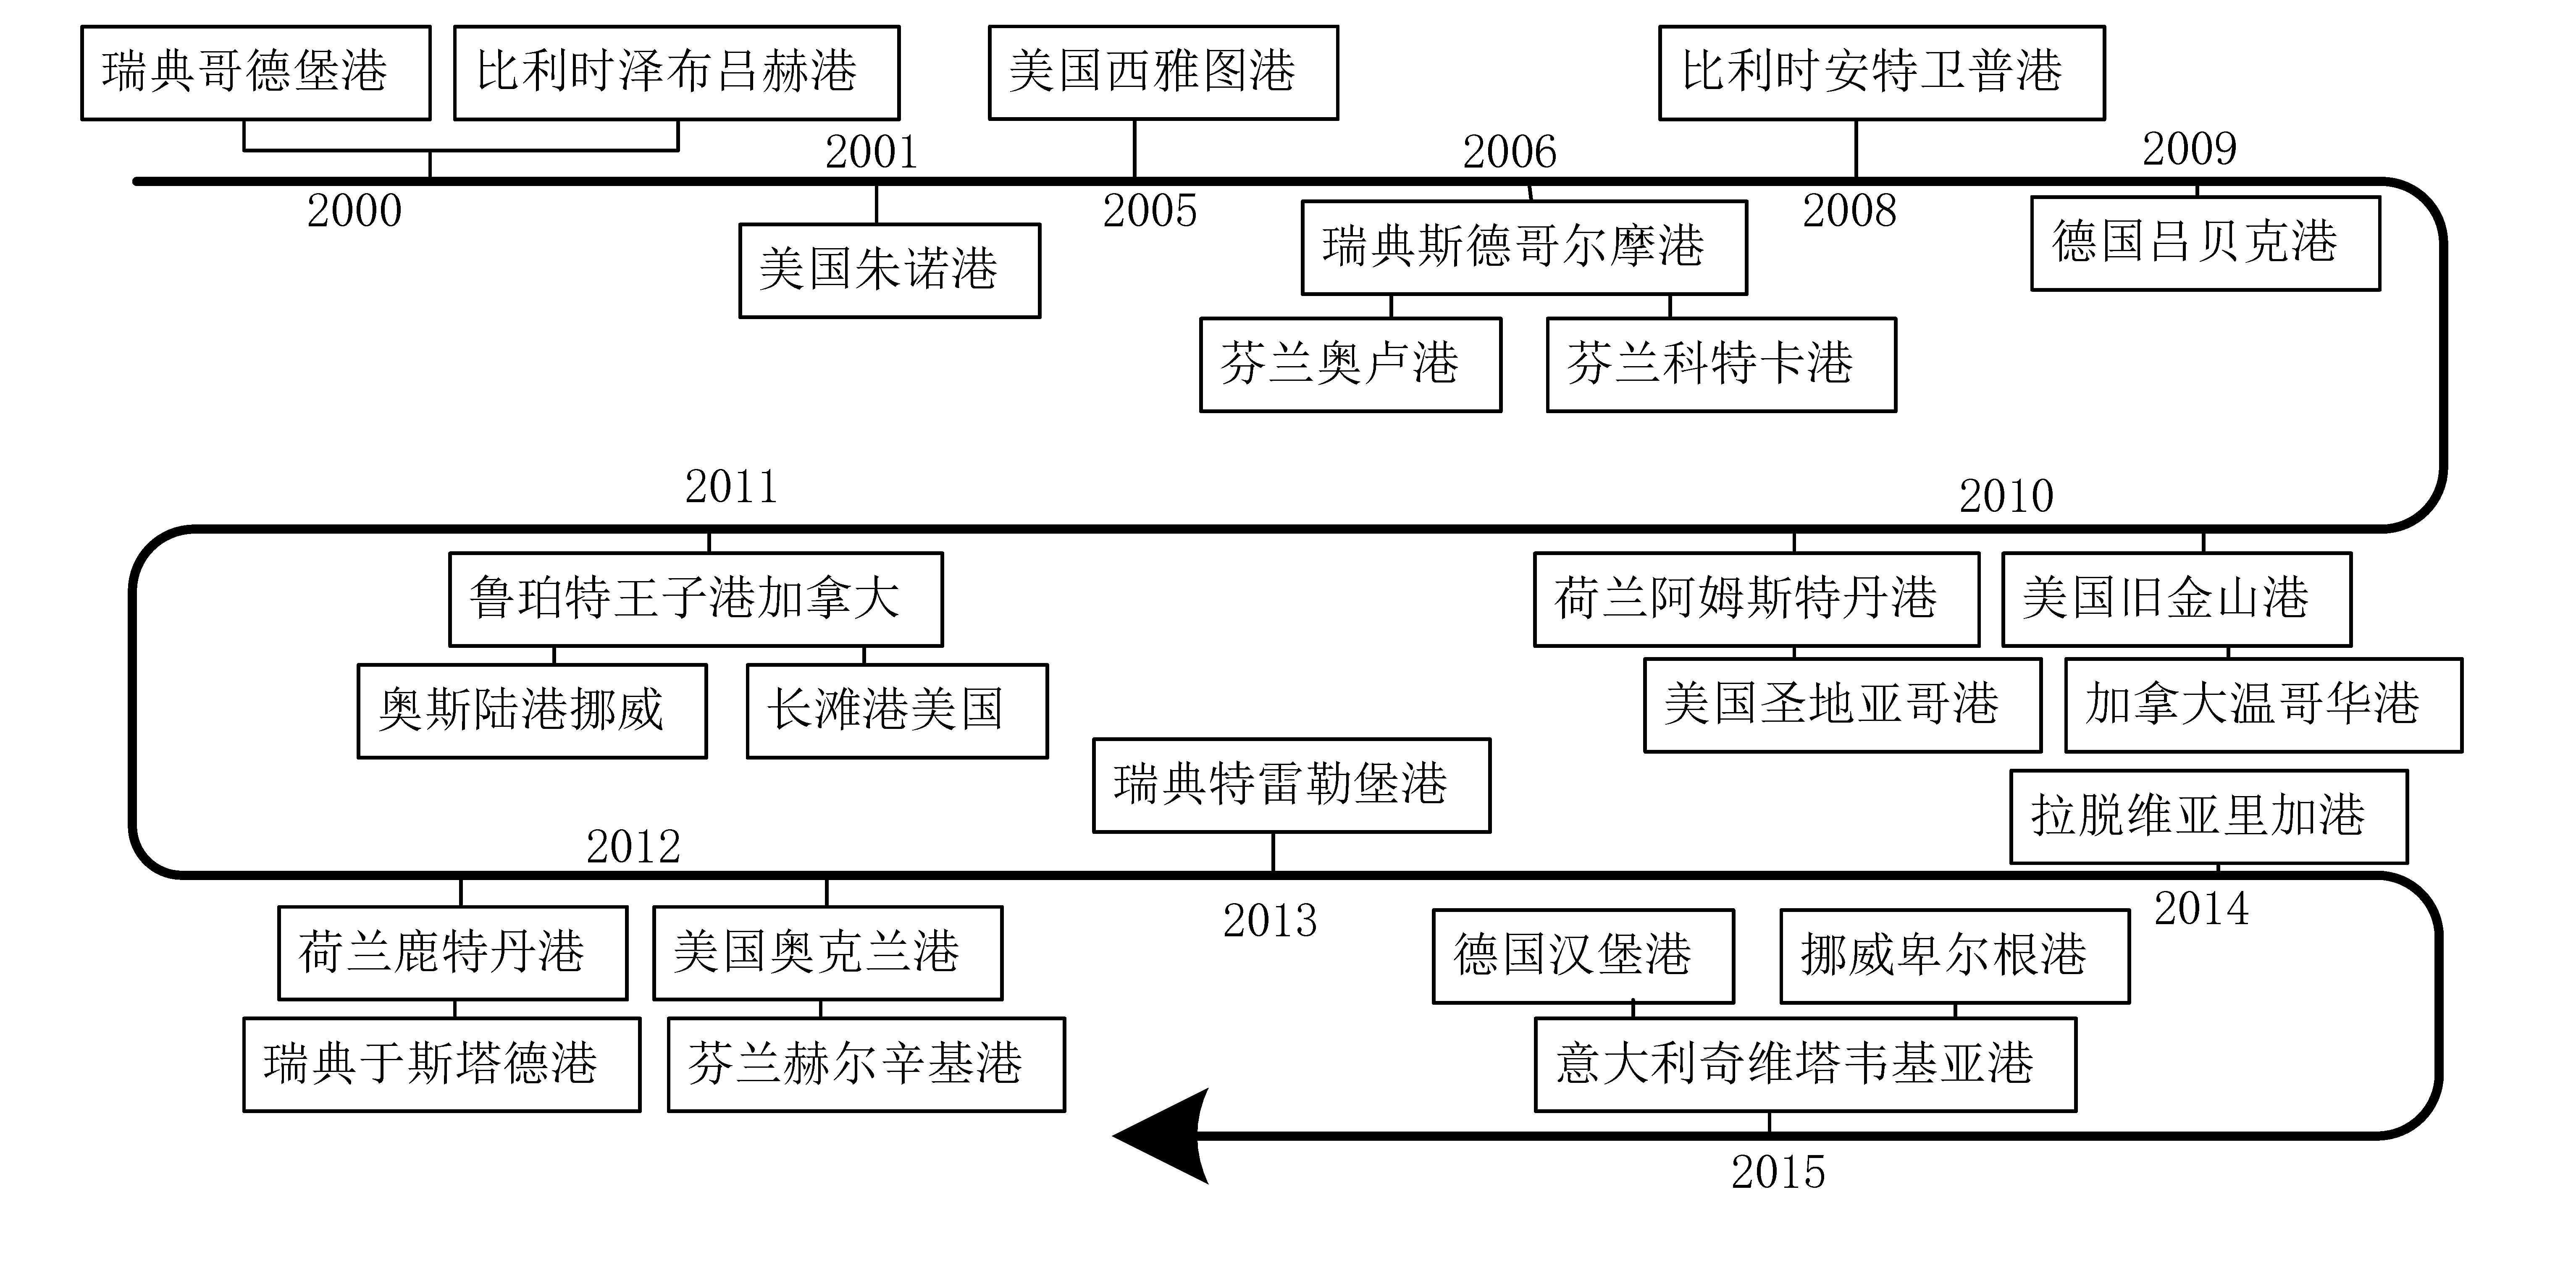
\includegraphics[width=\textwidth]{chapter1/国外应用岸电技术的主要港口.pdf}
	\caption{国外主要港口的岸电发展}
	\label{fig:国外主要港口的岸电发展}
\end{figure}

图\ref{fig:国外主要港口的岸电发展},表示了国外主要港口的岸电发展和建设情况。总之,发达国家主要港口的岸电系统建设和应用已经比较普
遍,而且像ABB、西门子和凯福特一些西方发达国家的大公司拥有岸电系统总体建设的能力,他们拥有较大的技术领先优势,产品成熟而且
掌握大量岸电系统核心技术与专利,如凯福特的电源管理系统和快速连接头,ABB公司的静止频率变换器(PCS6000)\cite{SP5}。

\subsection{国内应用状况}

如图\ref{fig:国内主要港口的岸电发展}所示,我们可以看到近年来国内主要港口的岸电的建设情况。
我国最早对船舶岸电技术进行研究始于2005年,上海港开始对船舶岸电系统进行立项研究。2009年,我国第一个岸电系统
在青岛港建设完成,并在青岛港招商局集装箱码头为停靠船舶提供岸电,项目采用的是380V/50Hz的低压方案,容量仅为131.6\si{kV.A}。
2010年,上海外高桥码头10kV/50Hz岸电系统建设完成,拥有了对集装箱船供应岸电的能力。同年,连云港港建成了高压/低压岸电系统,
是国内首例实现了高压上船的项目,并成功将其应用在“中韩之星”客货两用船上\cite{SP4}。
此套岸电系统具有使用方便、整体轻巧,连接时间较短、实用性强等特点,获得了节能减排岸电专项奖和绿色港口技术认定\cite{SP8}。
后于2011年9月,连云港港为“富强中国”号开发了另一套船舶岸电系统,仍采取高压上船方案。

2012年,深圳蛇口集装箱码头完成了对低压和高压岸电系统的建设工作;
2013年,国内首次实现带电并网的岸电系统——神华集团高压上船岸电项目,完成调试\cite{SP8};
2014年,天津港太平洋码的“太平洋东二、东四泊位岸基船舶供电项目”建设完成,输入10kV/50Hz经变换后输出6.6kV/60HZ的交流电;
2015年,日照港建成了第一套民用高压岸电系统\cite{SP9},同年泰州靖江新华港岸电系统开始为散货船供电;
2016年,盐田港由德国西门子研发的高压岸电项目建成,项目设计容量3000kW,预计能够实现年电能替代量
150万\si{kW.h},减排约1000吨。同年5月,舟山港与国网公司合作的舟山港项目正式投运,采用高压上船方案,设计容量为
2和3\si{MV.A},可为船舶提供6.6kV/60Hz与6kV/50Hz的交流电\cite{SP10}。

2017年,交通运输部水运局发布的《港口岸电布局方案》计划要于2020年实现泊位100\%的岸电覆盖率,对促进我国岸电系统的应用发挥了重要作用。
2018年,日照港对2个泊位进行的岸电改造项目建成,到2018年底国内已建成约3700个岸电设施,覆盖约5200个供电泊位。
2019年,大铲湾码头实现了100\%的泊位岸电覆盖率,是我国华南地区首个实现岸电100\%覆盖率的集装箱码头\cite{SP11}。
截至2019年底,全国已建成港口岸电设施5400多套,覆盖泊位7000多个(含水上服务区),总体完成率达81\%\cite{SP12}。

\begin{figure}[!htp]
	\centering
	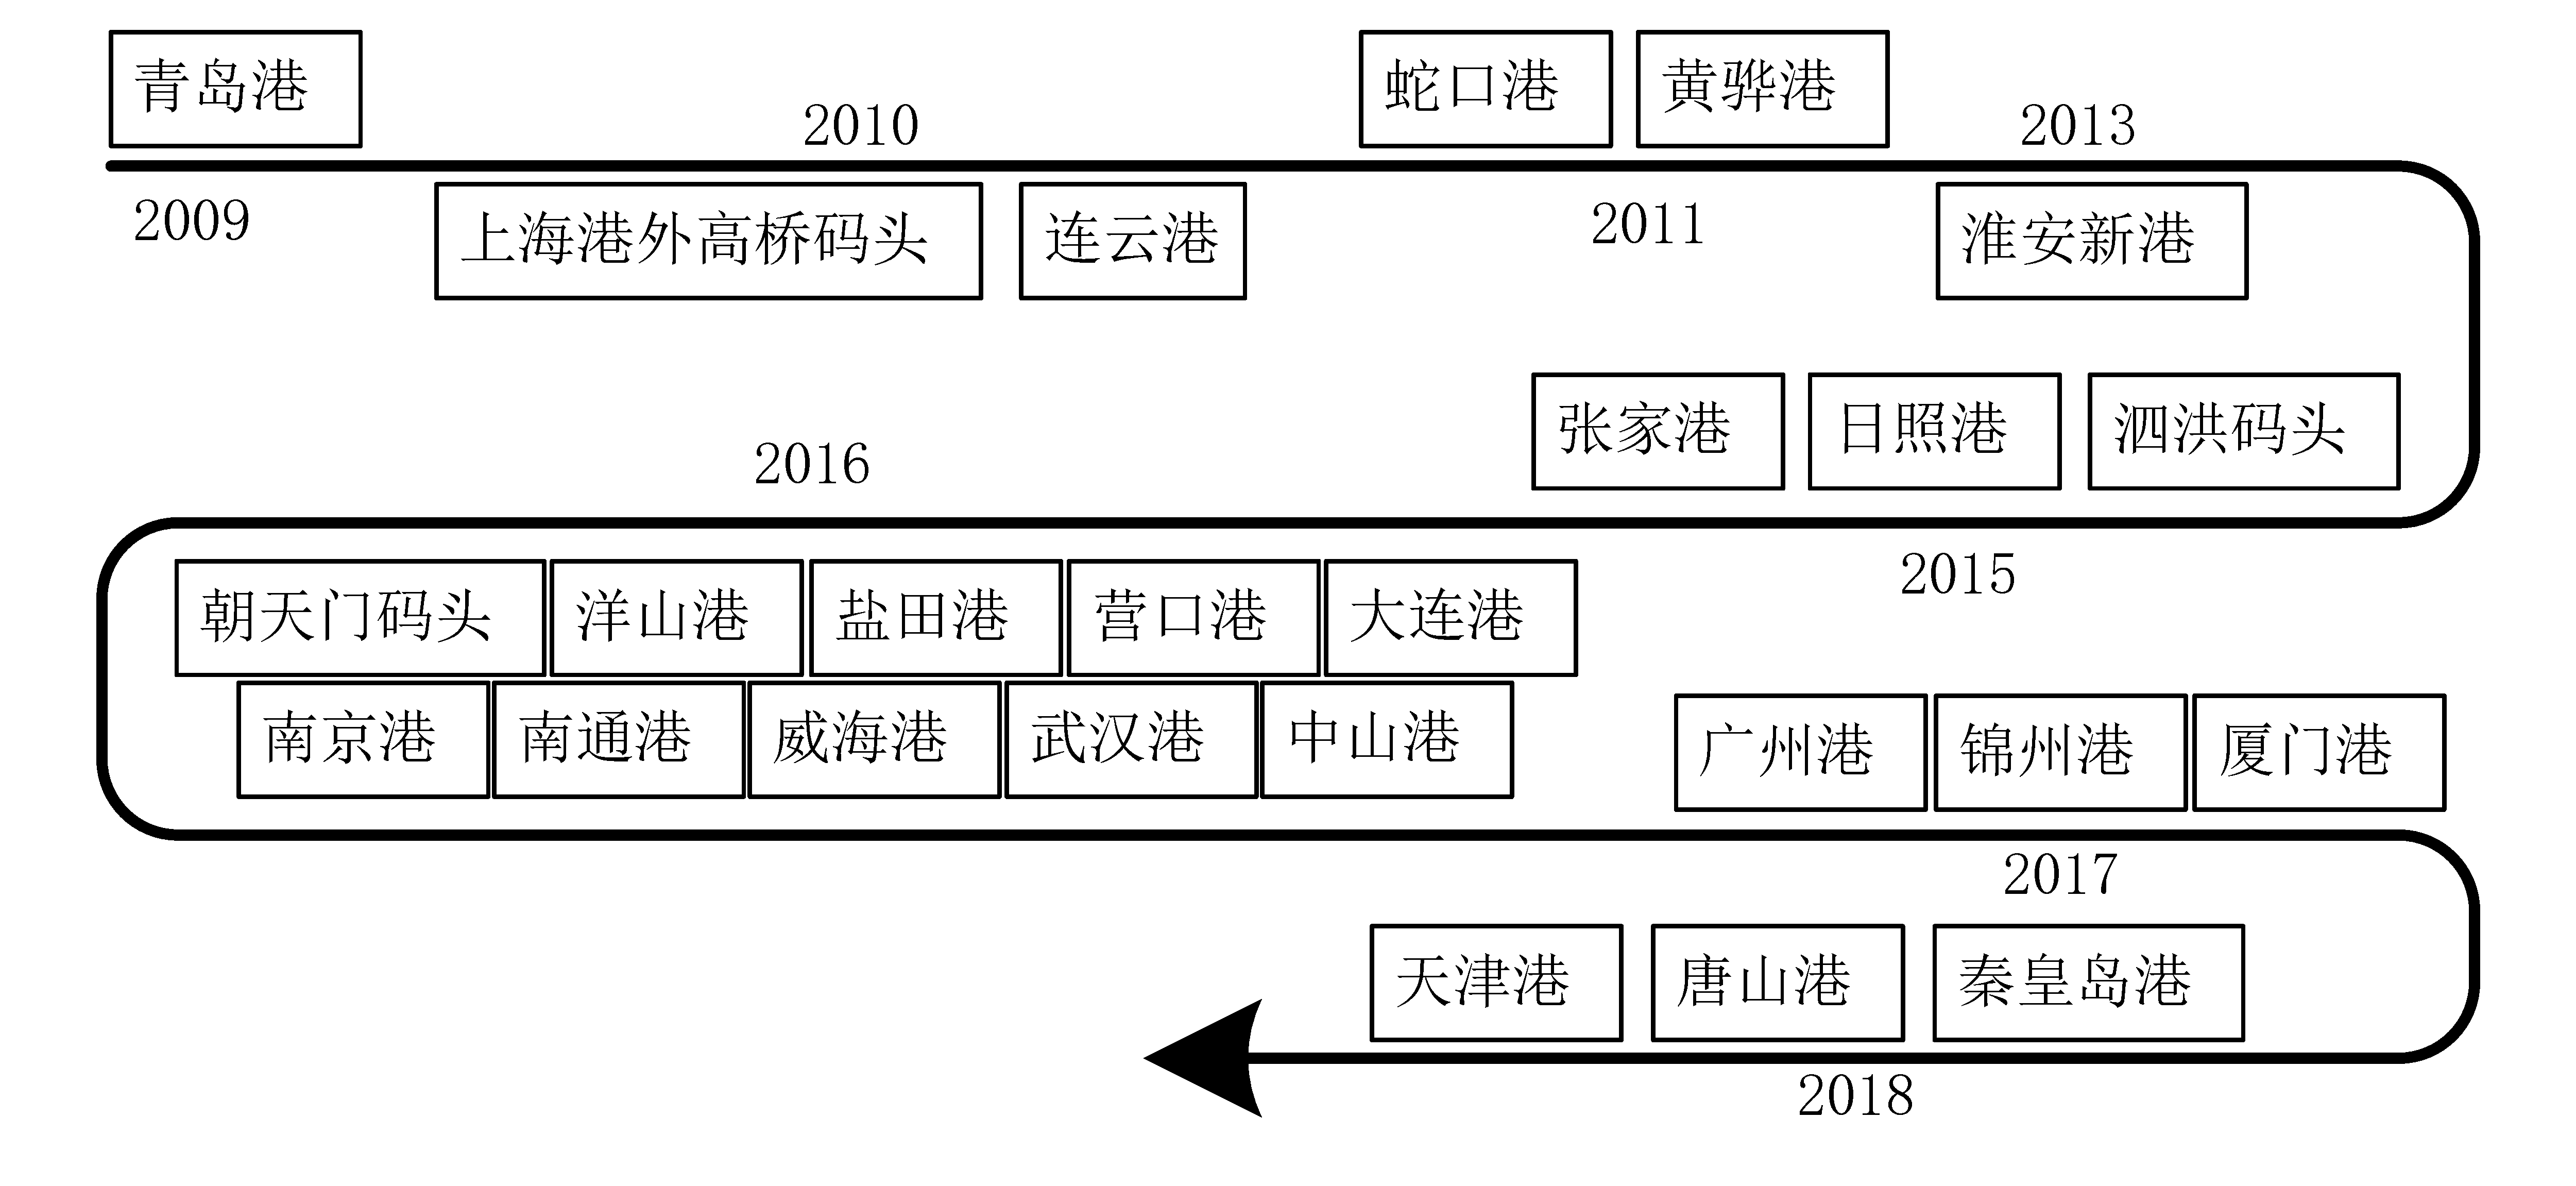
\includegraphics[width=0.9\textwidth]{chapter1/国内应用岸电技术的主要港口.pdf}
	\caption{国内主要港口的岸电发展}
	\label{fig:国内主要港口的岸电发展}
\end{figure}

2020年中国的岸电建设取得了阶段性的成果,由于西方国家的工业进程总体领先我国,其对船岸连接技术的早研发早应用使得其目前仍
处于行业领先地位。我国船岸连接技术应用起步晚,岸电普及率相对较低,近年来在交通运输部等政府部门与国网公司等企业的大力倡导
和积极推动下,国内一些港口已经具备了提供岸电能力。
据公开数据统计,截至2020年底集装箱船、滚装客船、邮轮、客船(3000吨以上载重)和干舱(50000吨以上载重)泊位
的岸电系统分布情况如图\ref{fig:中国岸电分布图}所示。

\begin{figure}[!htp]
	\centering
	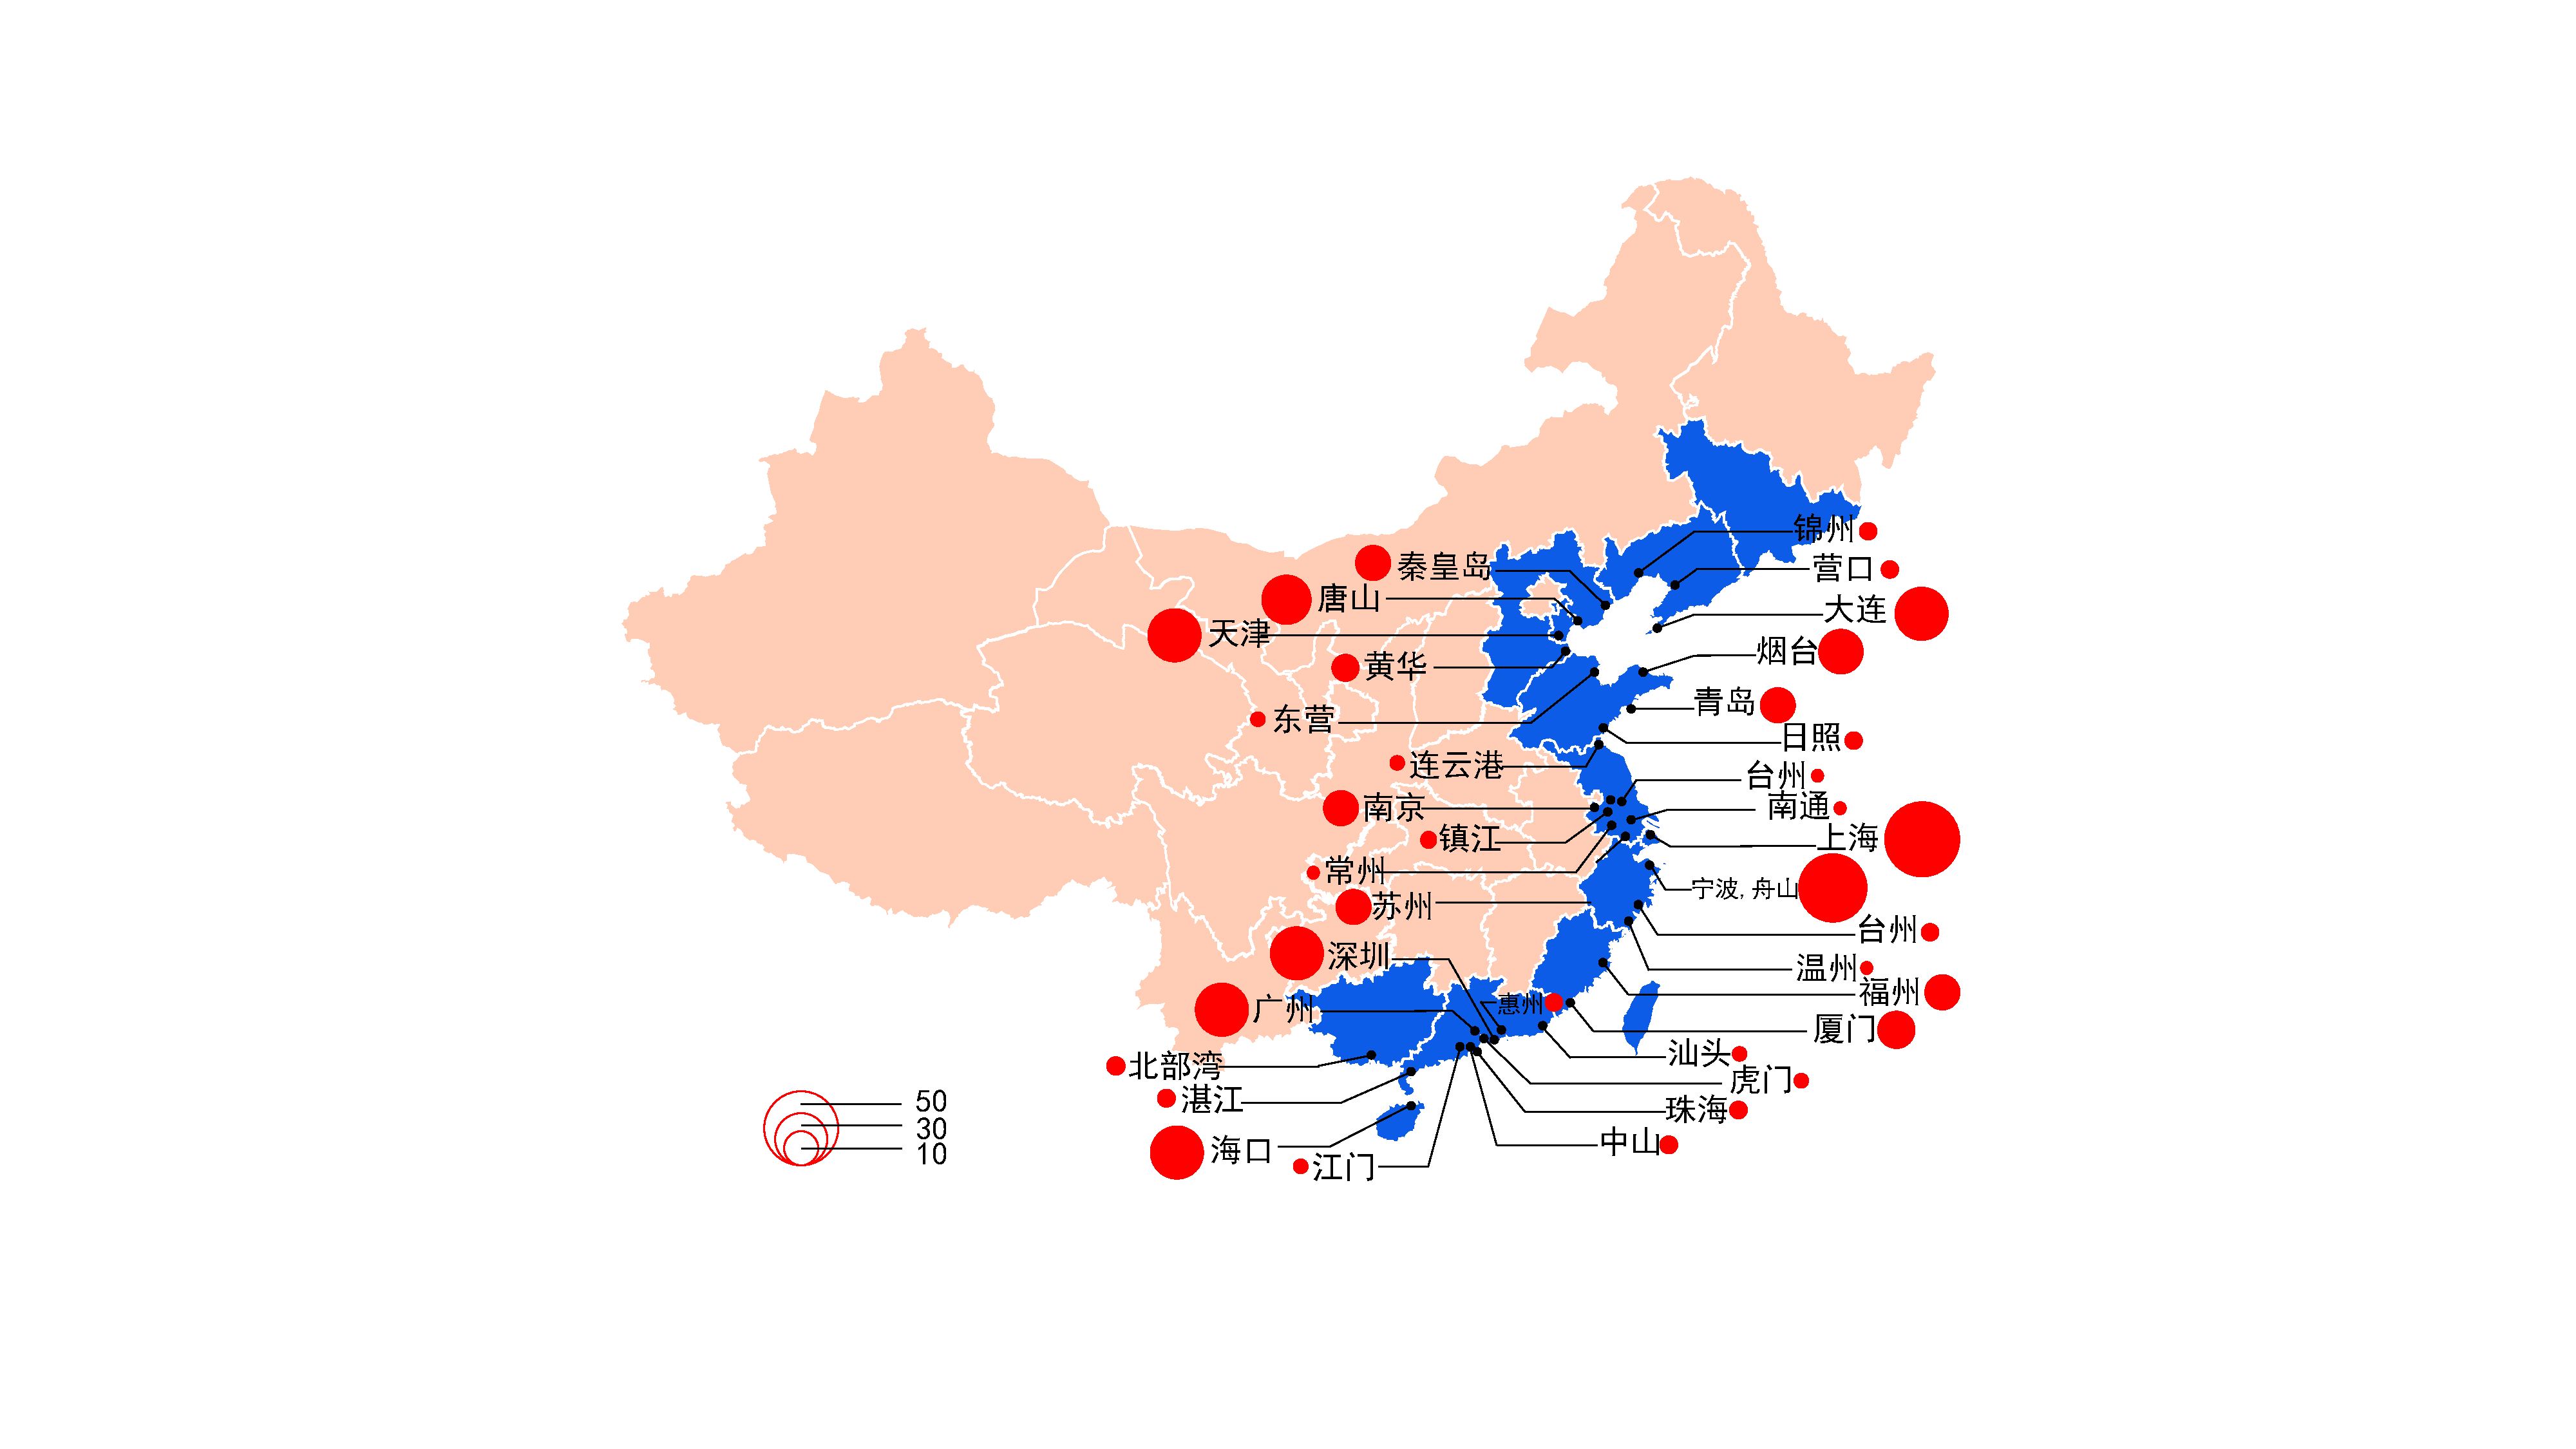
\includegraphics[width=0.9\textwidth]{chapter1/中国岸电分布图.pdf}
	\caption{ 2020年中国沿海地区岸电分布图}
	\label{fig:中国岸电分布图}
\end{figure}

此外,我国内陆沿长江流域的港口岸电发展也十分迅速\cite{SP17}。四川泸州港自2017年岸电系统投运以来,靠港船舶月平均用电量超过1万
千瓦时,累计使用电量30余万千瓦时,相当于减少废气排放3.21吨,为来往货船节约经济成本60余万元。
截至2020年10月,我国东部沿海地区29个重点港口码头已建成投运岸电设施97套,京杭大运河沿线码头和水上服务区共建成
投运岸电设施195套,基本实现全覆盖。

最近10年,我国岸电系统的发展迅速,国家重视程度很高,可以说我国的船岸连接系统的发展和应用正在如火如荼的进行着,当然也存在着一些
发展的问题如,泊位不足,运营经验有限,标准制定相关问题,但是中国拥有较大的市场容量,发展前景十分广阔。

\subsection{国内外岸电标准}

1983年,国际标准化组织(ISO)了ISO6812:1983 Preview Roll on/Roll off ship-to-shore connection,规定了滚装船的岸电设计标准。
这是第一个岸电系统领域的标准,也一直被沿用至今,后于2008年,ISO对该标准进行了重新审订\cite{SP4}。
表\ref{tab:国外相关标准的制定情况}中给出了国外岸电相关标准的制定情况与部分内容。

\begin{table}[!htp]
	\centering
	\caption[国外相关标准的制定情况]{国外相关标准的制定情况}
	\label{tab:国外相关标准的制定情况}
	\resizebox{0.85\textwidth}{!}{
	\begin{tabular}{c}
		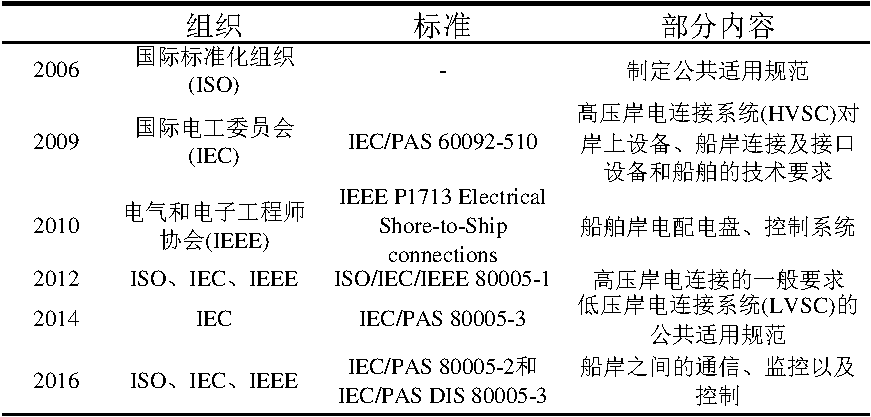
\includegraphics{chapter1/国外相关标准的制定情况.pdf} 
	\end{tabular}
	}
\end{table}

相比之下国内的岸电系统标准制定工作起步较晚,我国国内岸电系统领域相关标准的制定一定程度地依赖于国际标准\cite{SP4},
2005年,中国曾经派出代表参加了IEC 60092-510岸电标准的制定。近年来,我国交通部和国网公司大力倡导建设港口岸电系统,
国网公司下属许多单位从事着岸电系统和设备研发与生产,民营企业也逐渐加入到岸电系统的设计与研发的工作。同时,岸电标准
的制定也在逐步完善之中。交通部水运科学研究院等单位制定了《码头船舶岸电设施工程技术规范》,以及国网电力科学院等单
位制定了岸电系统、用电计量等一些列相关的企业标准\cite{SP14}。表\ref{tab:国内相关标准的制定情况}为岸电系统中
国标准的制定情况。

\begin{table}[!htp]
	\centering
	\caption[国内相关标准的制定情况]{国内相关标准的制定情况}
	\label{tab:国内相关标准的制定情况}
	\resizebox{0.85\textwidth}{!}{
	\begin{tabular}{c}
		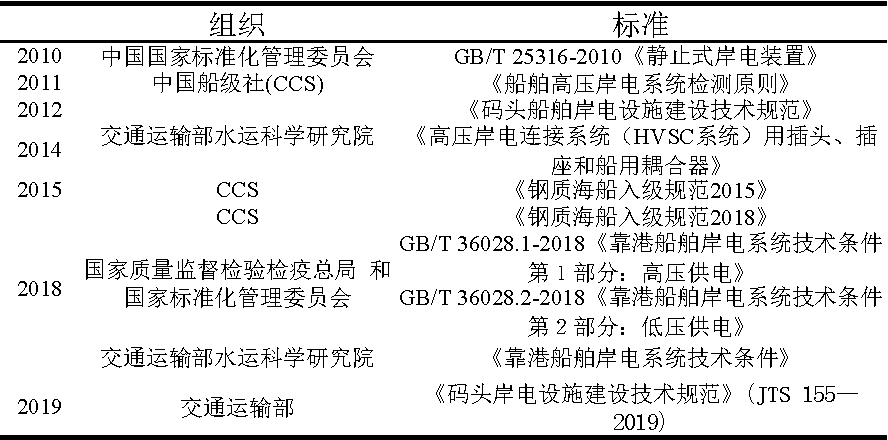
\includegraphics{chapter1/国内相关标准的制定情况.pdf} 
	\end{tabular}
	}
\end{table}

围绕标准化需求,当前国际国内相关标准化组织已开展了大量工作,对高压和低压岸电的通用要求、建设施工、连接设备等
提出了具体的要求。下一步,要结合实践需求,首先着眼于构建港口船舶岸电系统技术标准体系,覆盖低压、中压、高压岸
电,以及岸电系统的设计、建设、使用、维护和检测全流程,形成结构合理、专业配套、层次分明、划分明确的港口船舶岸
电标准体系表,明确标准缺项,用于指导和规范港口船舶岸电标准化工作。同时,加紧推进针对中压岸电,岸电系统检测试
验方法、综合管理、操作规程,以及连接系统具体设备要求和数据传输等关键领域的国内标准制修订工作,积极参与国际标
准化工作,提出国际标准新项目提案\cite{SP18}。

\section{论文研究内容及工作}
本文的研究目标旨在深入研究船舶岸电系统,并在此基础上设计船舶岸电并网控制的算法,以满足并网需求,做好保护功能
系统。使岸电系统可以实现港口岸电与船舶电网的无缝切换、负载的快速平稳转移以及相应的保护功能。本文的主要工作内容如下:

第一章,

第二章,

第三章,

第四章,

第五章,

第六章,



	\chapter{船岸连接基础知识}

\section{测试}

\subsection{测试}
	\chapter{船岸连接系统关键技术问题与分析}

\section{船用岸电电源系统结构与模型}

\subsection{船舶岸电电源结构}

岸电系统分为高压和低压两类,其中最关键的部分是岸电变频电源系统。岸电变频电源有不同的实现方案:1)高/低/高
,2)高/高。对比已知的岸电电源的拓扑结构,三相PWM整流与三相PWM逆变拓扑结构是目前最好的选择之一,变频电源
拓扑结构如图\ref{fig:岸电电源变流系统}所示。

\begin{figure}[!htp]
	\centering
	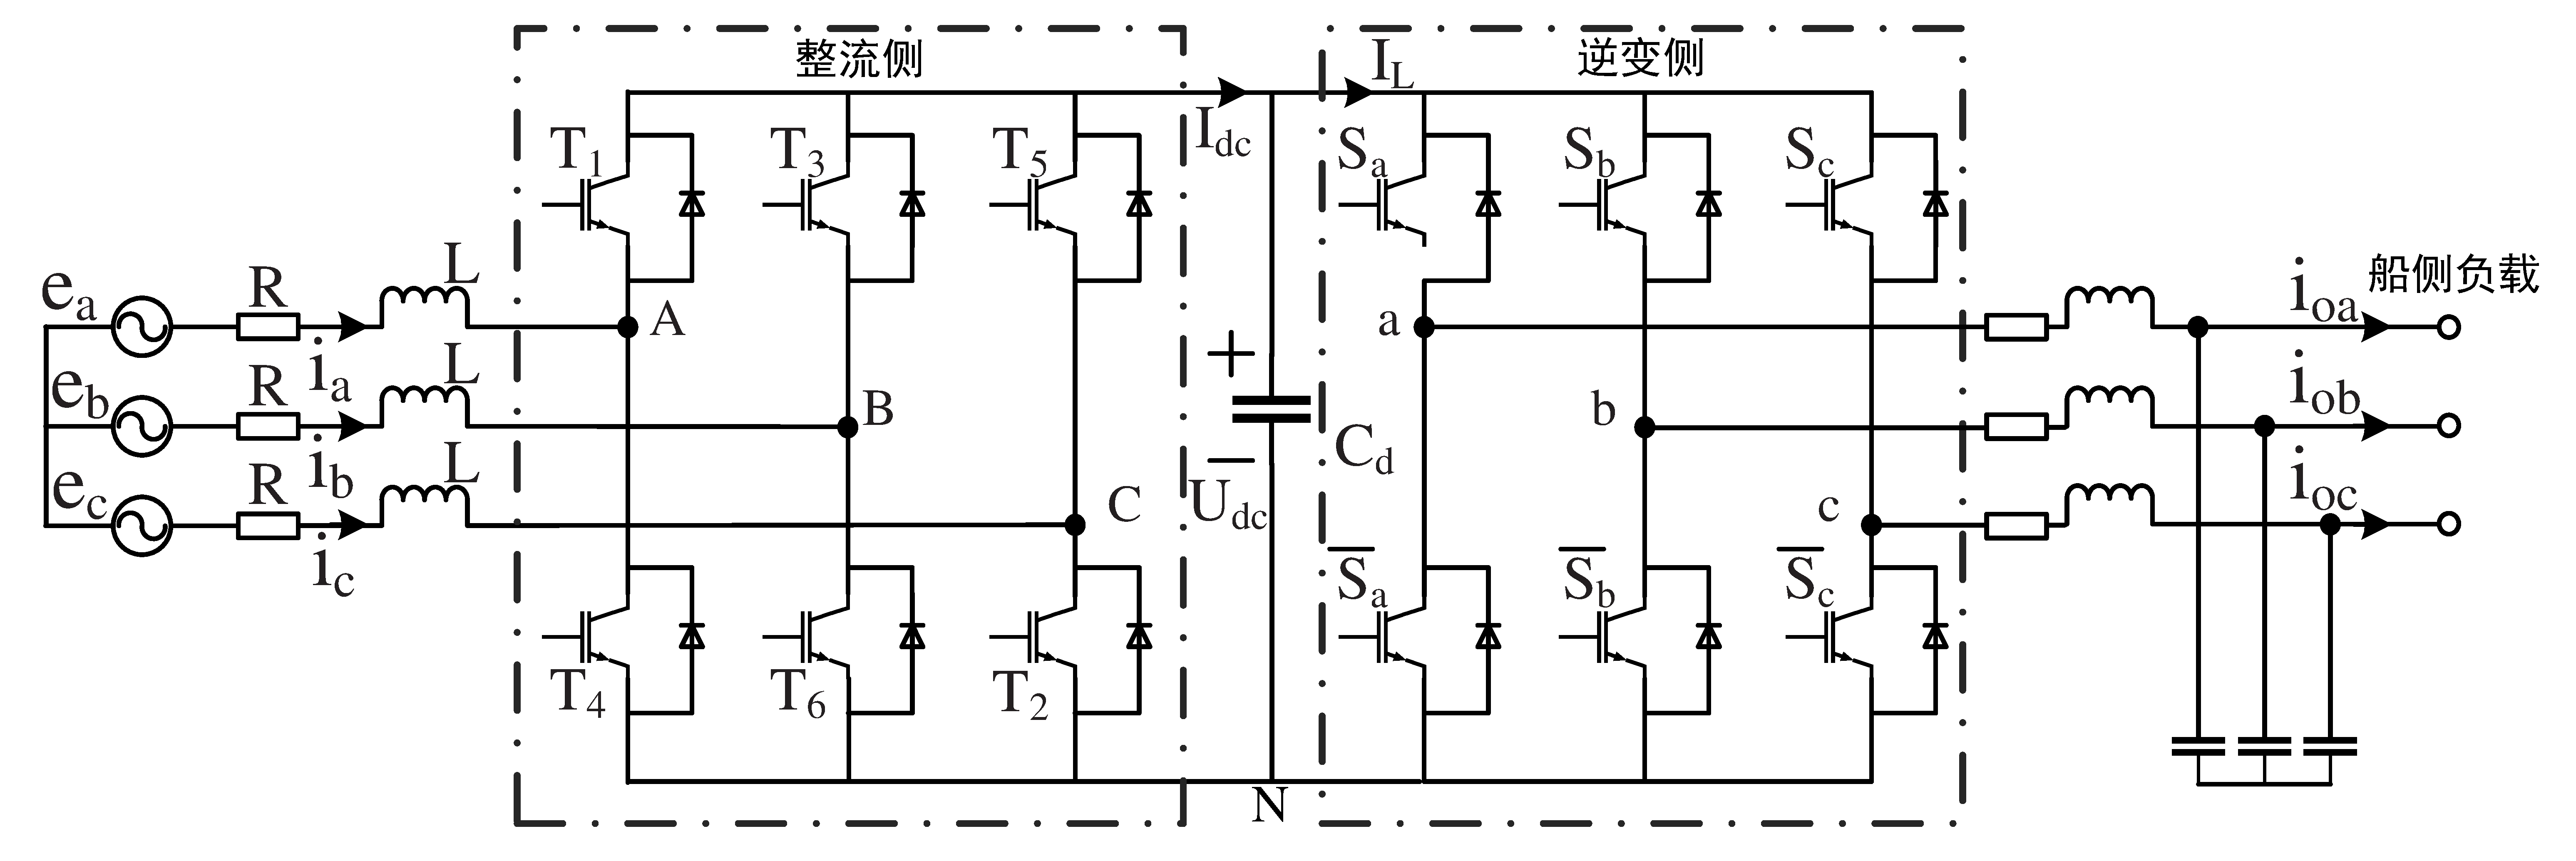
\includegraphics[width=\textwidth]{chapter3/变流器拓扑.pdf}
	\caption{岸电电源变流系统}
	\label{fig:岸电电源变流系统}
\end{figure}

\subsection{变流器整流侧模型}

整流侧为四象限有源PWM整流,采用先进成熟的IGBT技术,具有网侧谐波小、功率因数大和四象限运行的优点,
其拓扑结构如图\ref{fig:三相VSR拓扑结构图}所示。

\begin{figure}[!htp]
	\centering
	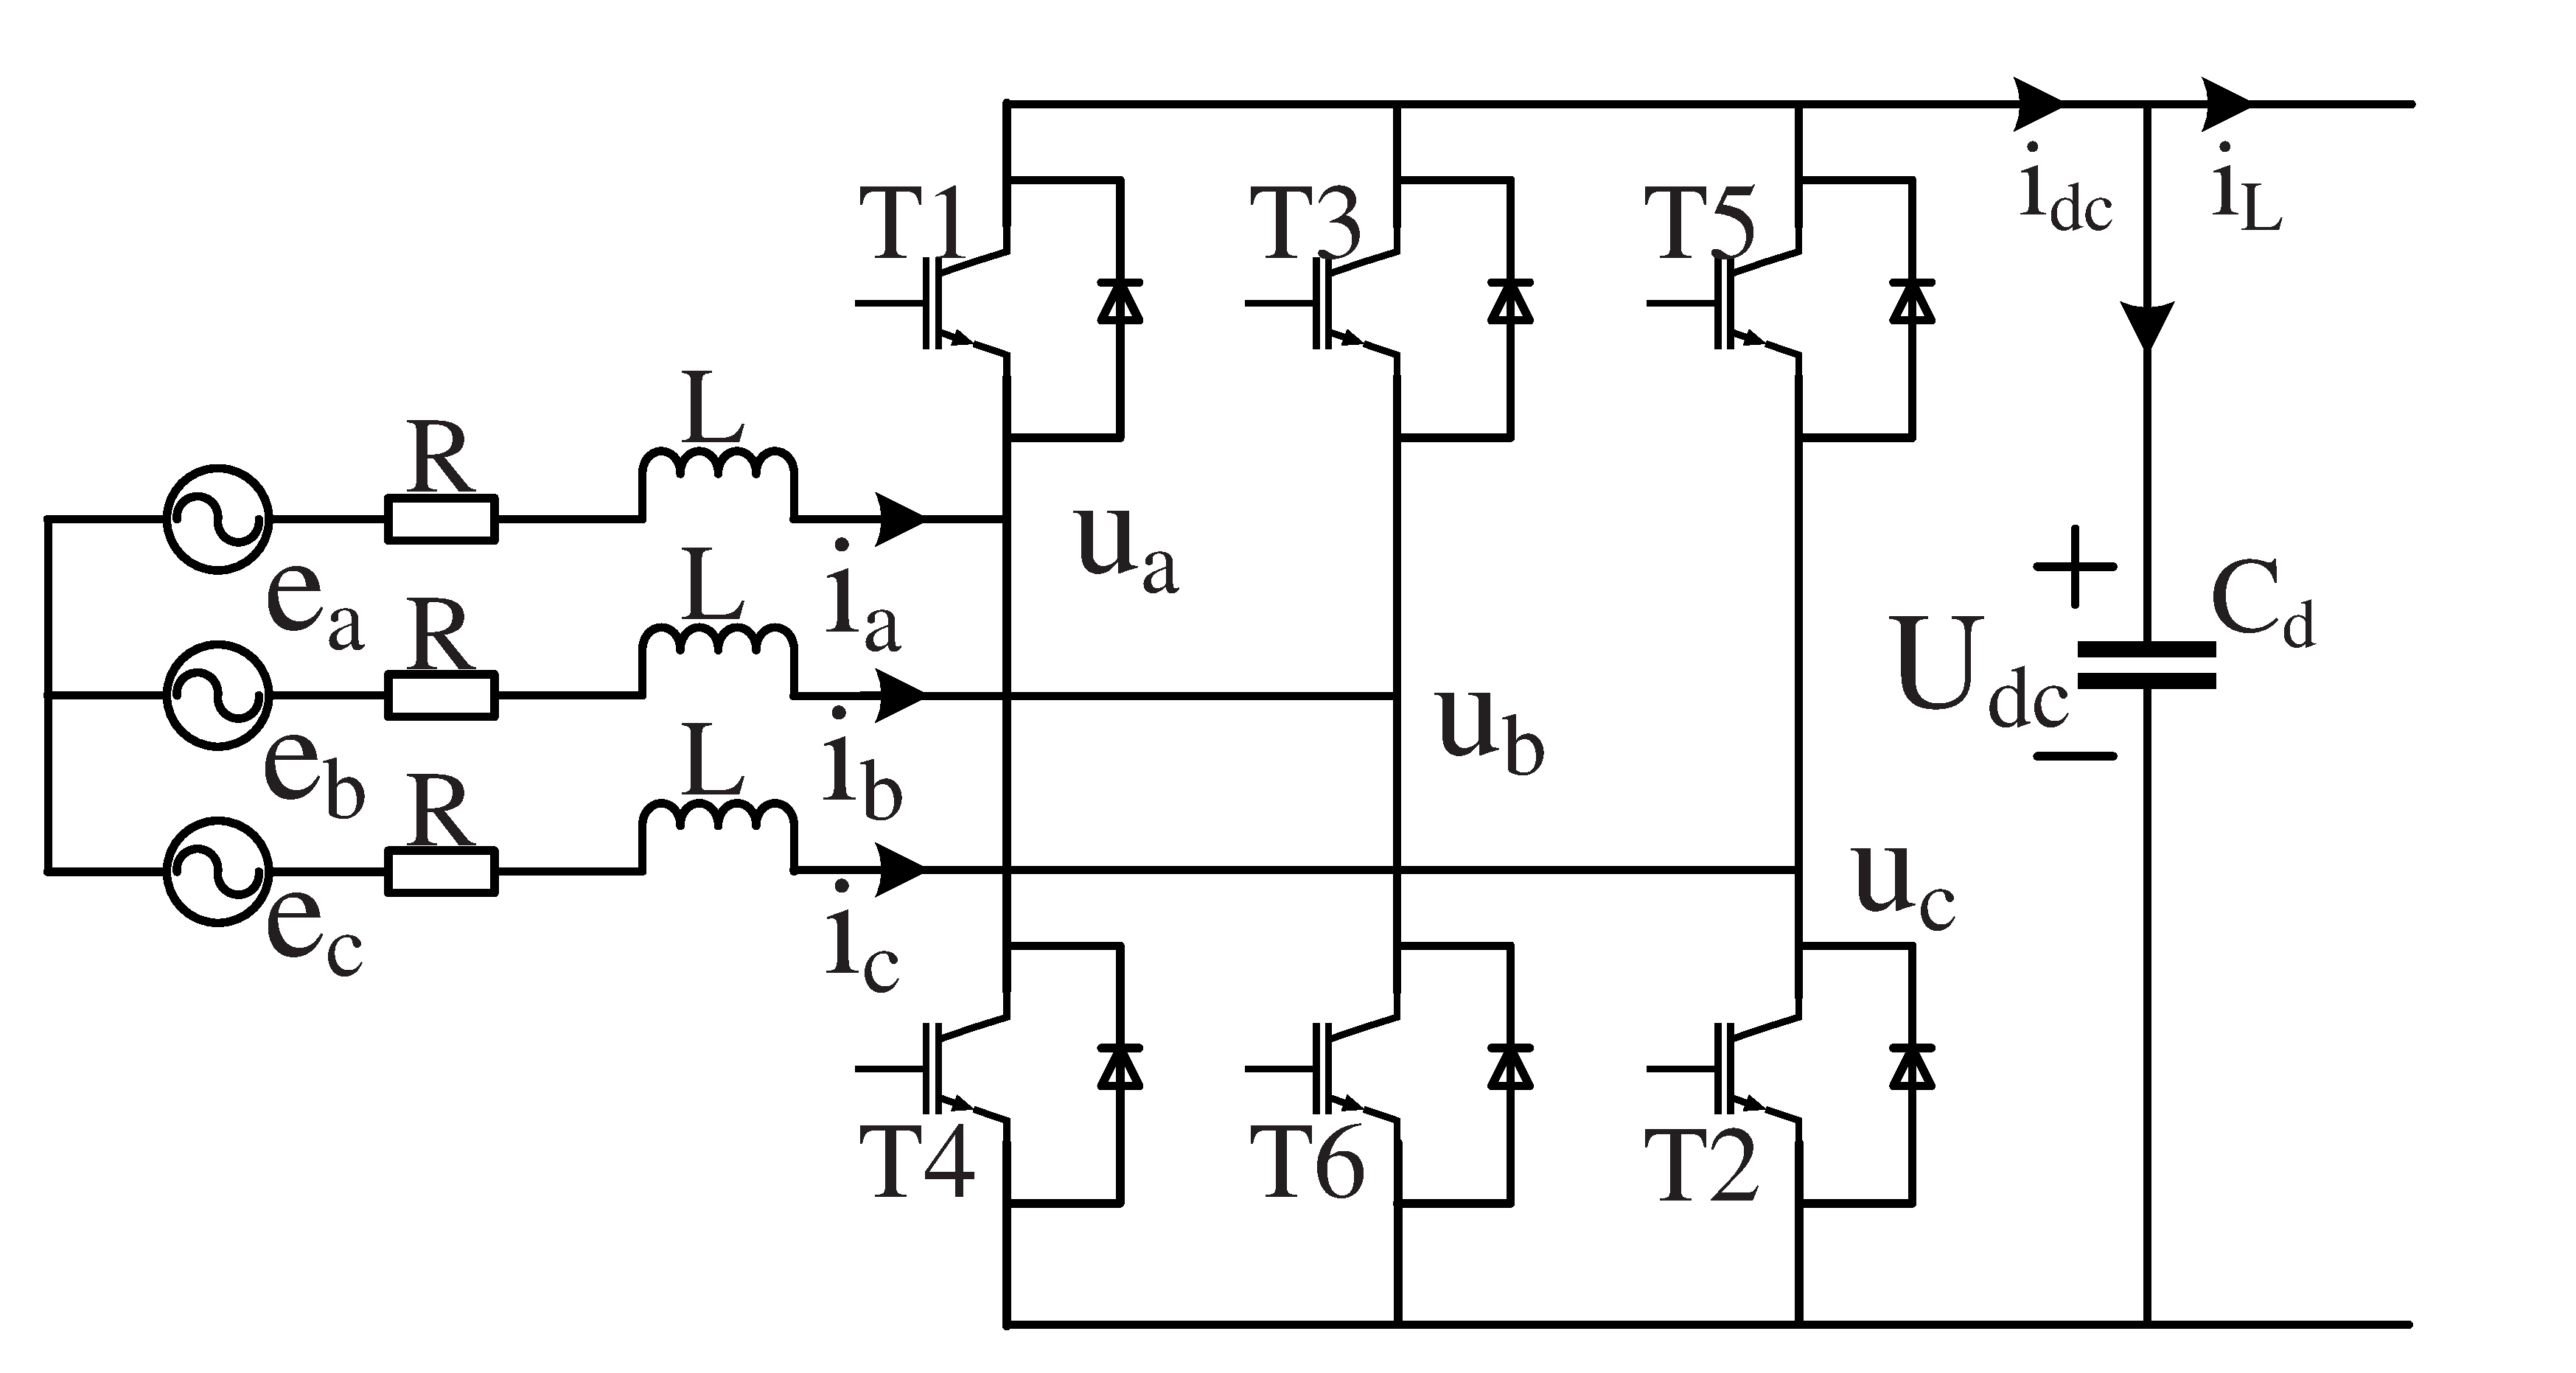
\includegraphics[width=0.65\textwidth]{chapter3/VSR/VSR拓扑.pdf}
	\caption{三相VSR拓扑结构图}
	\label{fig:三相VSR拓扑结构图}
\end{figure}

图\ref{fig:三相VSR拓扑结构图}中,$e_{k} \quad i_{k} \quad (k=u,v,w)$为网侧电压和电流,
理想情况下为正弦波。$i_{dc},i_{L},L,R,C$分别为直流侧电流,负载电流,滤波电感电流,网侧等效损耗电阻和
直流稳压电容。

对于IGBT功率开关定义开关函数$s_{k}$:
\begin{equation}
	s_{k} =
	\begin{cases}
		1 \quad \text{上桥臂IGBT导通,下桥臂IGBT关断} \\
		0 \quad \text{上桥臂IGBT关断,下桥臂IGBT导通} \\
	\end{cases}
	(k=u,v,w)
	\label{equ:SkR}
\end{equation}
根据基尔霍夫电压定律列写以下基本方程:
\begin{equation}
	\begin{cases}
		L\frac{di_{u}}{dt}+Ri_{u}=e_{u}-(u_{uN}+u_{NO})	\\
		L\frac{di_{v}}{dt}+Ri_{v}=e_{v}-(u_{vN}+u_{NO})	\\
		L\frac{di_{w}}{dt}+Ri_{w}=e_{w}-(u_{wN}+u_{NO})	\\
	\end{cases}
\end{equation}
又因为$u_{kN}=u_{dc}s_{k} \quad (k=u,v,w)$,所以有:
\begin{equation}
	\begin{cases}
		L\frac{di_{u}}{dt}+Ri_{u}=e_{u}-(u_{dc}s_{u}+u_{NO}) \\
		L\frac{di_{v}}{dt}+Ri_{v}=e_{v}-(u_{dc}s_{v}+u_{NO}) \\
		L\frac{di_{w}}{dt}+Ri_{w}=e_{w}-(u_{dc}s_{w}+u_{NO}) \\
	\end{cases}
	\label{equ:3-3}
\end{equation}
三相对称,所以有:
\begin{equation}
	\begin{cases}
		e_{u}+e_{v}+e_{w}=0	\\
		i_{u}+i_{v}+i_{w}=0 \\
	\end{cases}
	\label{equ:3-6}
\end{equation}
将式(\ref{equ:3-6})代入式(\ref{equ:3-3})中得:
\begin{equation}
	u_{NO}=-\frac{u_{dc}}{3} \left ( s_{u}+s_{v}+s_{w}  \right )
\end{equation}
直流侧电流$i_{dc}$可以表示为:
\begin{equation}
	i_{dc}=i_{u}s_{u}+i_{v}s_{w}+i_{w}s_{w}
\end{equation}
由基尔霍夫电流定律,直流侧电容电流为:
\begin{equation}
	C\frac{du_{dc}}{dt}=i_{u}s_{u}+i_{v}s_{w}+i_{w}s_{w}-i_{L}
\end{equation}

设状态变量$\boldsymbol{X}=[i_{u},i_{v},i_{w},u_{dc}]^{T}$,
输入变量$\boldsymbol{U}=[e_{u},e_{v},e_{w},i_{L}]^{T}$则三项VSR状态空间可以表示为:

\begin{equation}
	\boldsymbol{\dot{X}}=\boldsymbol{AX}+\boldsymbol{BU}
	\label{equ:VSR状态空间}
\end{equation}
上式中:
\begin{equation}
	\boldsymbol{A}=
	\begin{pmatrix}
		-\frac{R}{L}    & 0               & 0               & -\frac{1}{L}  ( s_{u}-\frac{1}{3} \sum\limits_{k=u,v,w} s_{k}  ) \\
		0               & -\frac{R}{L}    & 0               & -\frac{1}{L}  ( s_{u}-\frac{1}{3} \sum\limits_{k=u,v,w} s_{k}  ) \\
		0               & 0               & -\frac{R}{L}    & -\frac{1}{L}  ( s_{u}-\frac{1}{3} \sum\limits_{k=u,v,w} s_{k}  ) \\
		\frac{s_{a}}{C} & \frac{s_{b}}{C} & \frac{s_{c}}{C} & 0
	\end{pmatrix}
\end{equation}

\begin{equation}
	\boldsymbol{B}=
	\begin{pmatrix}
		\frac{1}{L} & 0           & 0           & 0            \\
		0           & \frac{1}{L} & 0           & 0            \\
		0           & 0           & \frac{1}{L} & 0            \\
		0           & 0           & 0           & -\frac{1}{C}
	\end{pmatrix}
\end{equation}

至此我们已经得到了VSR在abc坐标系下的数学模型,模型的物理意义清晰,但是网侧为正弦量不利于控制系统的设计。
我们可以利用坐标变换理论将abc坐标系下的模型转换为同步旋转dq坐标系下的模型,经变换后的网侧正弦量变为了
直流量,从而方便控制系统的设计。

将abc坐标系的VSR模型转换为dq坐标系模型前,我们需要首先将abc坐标系转换为两相静止$\alpha\beta$坐标系。
设有通用的三相交流矢量$\boldsymbol{X}$,我们使a轴与$\alpha$轴重合,则有。

\begin{equation}
	\begin{pmatrix}
		x_{\alpha } \\
		x_{\beta }
	\end{pmatrix}
	=
	\frac{2}{3}
	\begin{pmatrix}
		1 & -\frac{1}{2}         & -\frac{1}{2}        \\
		0 & -\frac{\sqrt{3} }{2} & \frac{\sqrt{3} }{2}
	\end{pmatrix}
	\begin{pmatrix}
		x_{a} \\
		x_{b} \\
		x_{c}
	\end{pmatrix}
	\label{equ:abc2αβ}
\end{equation}
其中,$x_{\alpha}$、$x_{\beta}$为$\boldsymbol{X}$在$\alpha$、$\beta$轴上的投影,
$x_{a}$、$x_{b}$、$x_{c}$$\boldsymbol{X}$在a、b、c轴上的投影。

对于三相VSR有:
\begin{equation}
	\begin{cases}
		x_{k}\in  \{ e_{k},e_{k},s_{k} \} \quad(k=a,b,c)          \\
		x_{l}\in  \{ e_{l},e_{l},s_{l} \} \quad(l=\alpha ,\beta ) \\
		x_{j}\in  \{ e_{j},e_{j},s_{j} \} \quad(j=d,q)
	\end{cases}
\end{equation}
联立式(\ref{equ:abc2αβ}),式(\ref{equ:VSR状态空间})化简可得:
\begin{equation}
	\begin{cases}
		C \frac{\mathrm{d} u_{\mathrm{dc}}}{\mathrm{d} t}=\frac{3}{2}\left(i_{\alpha} s_{\alpha}+i_{\beta} s_{\beta}\right)-i_{\mathrm{L}} \\
		L \frac{\mathrm{d} i_{\alpha}}{\mathrm{d} t}+R i_{\alpha}=e_{\alpha}-u_{\mathrm{dc}} s_{\alpha}                                    \\
		L \frac{\mathrm{d} i_{\beta}}{\mathrm{d} t}+R i_{\beta}=e_{\beta}-u_{\mathrm{dc}} s_{\beta}
	\end{cases}
	\label{equ:3-17}
\end{equation}
αβ坐标系到dq坐标系的转换矩阵为:
\begin{equation}
	\begin{pmatrix}
		x_{\alpha } \\
		x_{\beta }
	\end{pmatrix}=
	\begin{pmatrix}
		cos\varphi & -sin\varphi \\
		sin\varphi & cos\varphi
	\end{pmatrix}
	\begin{pmatrix}
		x_{d } \\
		x_{q}
	\end{pmatrix}
	\label{equ:αβ2dq变换公式}
\end{equation}
其中,$\varphi$为d轴与$\alpha$轴的夹角。联立式(\ref{equ:αβ2dq变换公式}),式(\ref{equ:3-17})得:
\begin{equation}
	\begin{cases}
		C \frac{\mathrm{d} u_{\mathrm{dc}}}{\mathrm{d} t}=\frac{3}{2}\left(i_{\mathrm{d}} s_{\mathrm{d}}+i_{\mathrm{q}} s_{\mathrm{q}}\right)-i_{\mathrm{L}} \\
		L \frac{\mathrm{d} i_{\mathrm{d}}}{\mathrm{d} t}+R i_{\mathrm{d}}-\omega L i_{\mathrm{q}}=e_{\mathrm{d}}-u_{\mathrm{dc}} s_{\mathrm{d}}              \\
		L \frac{\mathrm{d} i_{\mathrm{q}}}{\mathrm{d} t}+R i_{\mathrm{q}}+\omega L i_{\mathrm{d}}=e_{\mathrm{q}}-u_{\mathrm{dc}} s_{\mathrm{q}}
	\end{cases}
	\label{equ:VSR dq数学模型}
\end{equation}
三相VSR dq数学模型的结构如图\ref{fig:三相VSR dq数学模型结构.pdf}所示:
\begin{figure}[!htp]
	\centering
	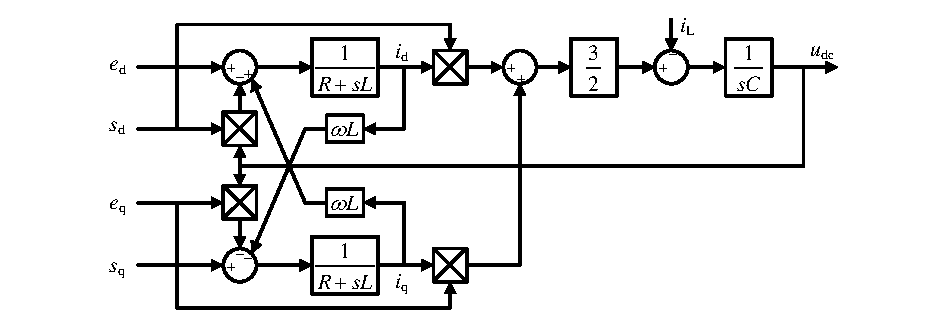
\includegraphics[width=\textwidth]{chapter3/VSR/三相VSR dq数学模型结构.pdf}
	\caption{三相VSR dq数学模型结构.pdf}
	\label{fig:三相VSR dq数学模型结构.pdf}
\end{figure}

\subsection{变流器逆变侧模型}

逆变侧采用PWM逆变,其拓扑结构如图\ref{fig:三相VSI拓扑结构图}所示。

\begin{figure}[!htp]
	\centering
	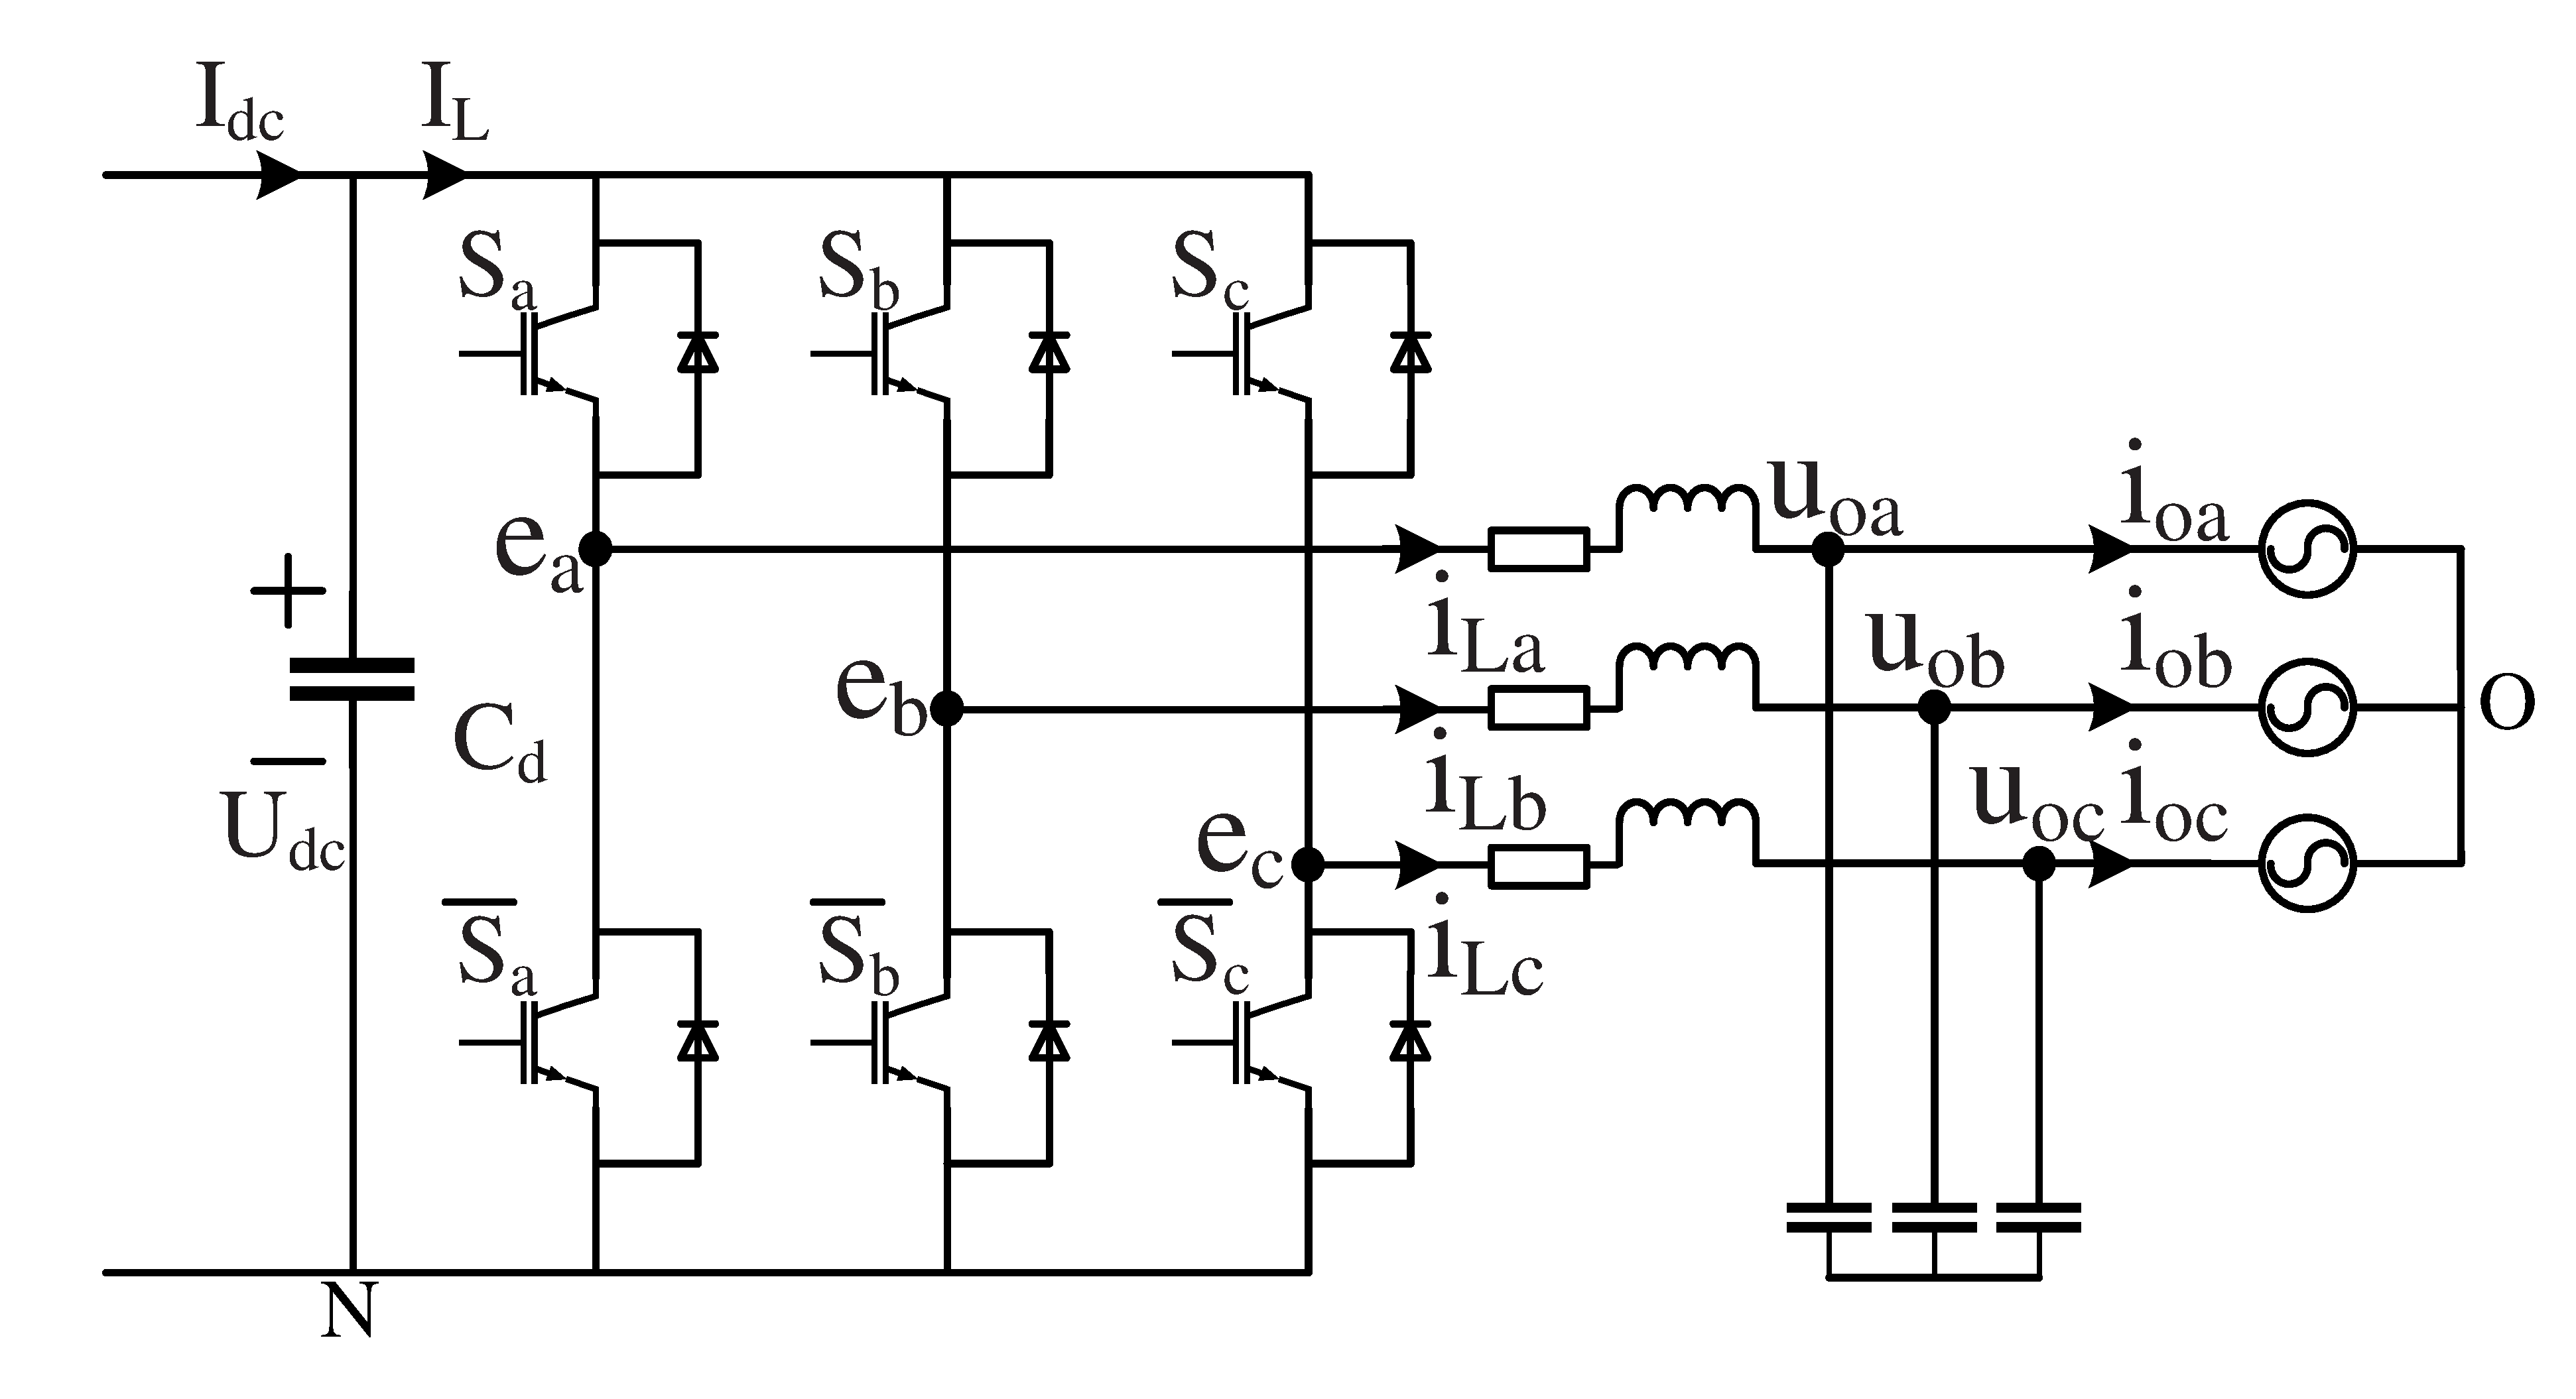
\includegraphics[width=0.65\textwidth]{chapter3/VSI/VSI拓扑.pdf}
	\caption{三相VSI拓扑结构图}
	\label{fig:三相VSI拓扑结构图}
\end{figure}
对于IGBT功率开关定义开关函数$s_j$:
\begin{equation}
	s_{j} =
	\begin{cases}
		1 \quad \text{上桥臂IGBT导通,下桥臂IGBT关断} \\
		0 \quad \text{上桥臂IGBT关断,下桥臂IGBT导通} \\
	\end{cases}
	(j=a,b,c)
	\label{equ:SkI}
\end{equation}
根据基尔霍夫电压定律列写回路方程:
\begin{equation}
	\begin{cases}
		L \frac{d i_{La}}{dt}+R i_{La}=e_{a}-u_{oa}-u_{ON} \\
		L \frac{d i_{Lb}}{dt}+R i_{Lb}=e_{b}-u_{ob}-u_{ON} \\
		L \frac{d i_{Lc}}{dt}+R i_{Lc}=e_{c}-u_{oc}-u_{ON}
	\end{cases}
	\label{equ:3-21}
\end{equation}
将$e_{k}=u_{dc}s_{k}\quad(k=a,b,c)$代入式(\ref{equ:3-21})得:
\begin{equation}
	\begin{cases}
		L\frac{di_{La}}{dt}+Ri_{La}=u_{dc}s_{a}-u_{oa}-u_{ON} \\
		L\frac{di_{Lb}}{dt}+Ri_{Lb}=u_{dc}s_{b}-u_{ob}-u_{ON} \\
		L\frac{di_{Lc}}{dt}+Ri_{Lc}=u_{dc}s_{c}-u_{oc}-u_{ON}
		\label{equ:VSI model1}
	\end{cases}
\end{equation}
考虑到三相对称性,则有:
\begin{equation}
	\begin{cases}
		i_{La}+i_{Lb}+i_{Lc}=0 \\
		u_{oa}+u_{ob}+u_{oc}=0 \\
	\end{cases}
	\label{equ:3-23}
\end{equation}
联立式(\ref{equ:VSI model1})和式(\ref{equ:3-23})得:
\begin{equation}
	u_{ON}=\frac{u_{dc}}{3}\sum_{k=a,b,c}s_{k}
\end{equation}
根据基尔霍夫电流定律建立整流侧电容电流方程和滤波电容节点处电流方程:
\begin{equation}
	\begin{cases}
		C\frac{du_{oa}}{dt}=i_{La}-i_{oa} \\
		C\frac{du_{ob}}{dt}=i_{Lb}-i_{ob} \\
		C\frac{du_{oc}}{dt}=i_{Lc}-i_{oc} \\
		C\frac{du_{dc}}{dt}=i_{dc}-i_{L}
	\end{cases}
\end{equation}

设状态变量$\boldsymbol{X}=[i_{La},i_{Lb},i_{Lc},u_{dc}]^{T}$,
输入变量$\boldsymbol{U}=[e_{oa},e_{ob},e_{oc},i_{L}]^{T}$则三项VSR状态方程可以表示为:
\begin{equation}
	\boldsymbol{\dot{X}}=\boldsymbol{A}\boldsymbol{X}+\boldsymbol{B}\boldsymbol{E}+\boldsymbol{Z}
\end{equation}
上式中:
\begin{equation}
	\boldsymbol{A}=
	\begin{pmatrix}
		-\frac{R}{L}    & 0               & 0               & - \frac{1}{3L} \sum\limits_{k=u,v,w} s_{k} \\
		0               & -\frac{R}{L}    & 0               & - \frac{1}{3L} \sum\limits_{k=u,v,w} s_{k} \\
		0               & 0               & -\frac{R}{L}    & - \frac{1}{3L} \sum\limits_{k=u,v,w} s_{k} \\
		\frac{s_{a}}{C} & \frac{s_{b}}{C} & \frac{s_{c}}{C} & 0
	\end{pmatrix}
\end{equation}

\begin{equation}
	\boldsymbol{B}=
	\begin{pmatrix}
		-\frac{1}{L} & 0            & 0            & 0            \\
		0            & -\frac{1}{L} & 0            & 0            \\
		0            & 0            & -\frac{1}{L} & 0            \\
		0            & 0            & 0            & -\frac{1}{C}
	\end{pmatrix}
\end{equation}

\begin{equation}
	\boldsymbol{Z}=
	\begin{pmatrix}
		0 & 0 & 0 & \frac{i_{dc}}{C}
	\end{pmatrix}^{T}
\end{equation}

与整流侧类似,为了得到三相VSI的dq数学模型,可以先将abc坐标系转换为$\alpha\beta$坐标系。
联立式(\ref{equ:abc2αβ})和式(\ref{equ:VSI model1})得到三相VSI的$\alpha\beta$数学模型:
\begin{equation}
	\begin{cases}
		L\frac{di_{L\alpha}}{dt}=-Ri_{L\alpha}+e_{\alpha}-u_{o\alpha} \\
		L\frac{di_{L\beta}}{dt}=-Ri_{L\beta}+e_{\beta}-u_{o\beta}
	\end{cases}
	\label{equ:VSI αβ model1}
\end{equation}

\begin{equation}
	\begin{cases}
		C\frac{du_{o\alpha}}{dt}=i_{L\alpha}-i_{o\alpha} \\
		C\frac{du_{o\beta}}{dt}=i_{L\beta}-i_{o\beta}
	\end{cases}
	\label{equ:VSI αβ model2}
\end{equation}

为使两相静止$\alpha\beta$坐标系转化为同步旋转dq坐标系,将式(\ref{equ:αβ2dq变换公式})代入
式(\ref{equ:VSI αβ model1})和式(\ref{equ:VSI αβ model2})中,整理得到VSI的dq模型:
\begin{equation}
	\begin{cases}
		L\frac{di_{Ld}}{dt}=-Ri_{Ld}+e_{d}+\omega Li_{Lq}-u_{od} \\
		L\frac{di_{Lq}}{dt}=-Ri_{Lq}+e_{q}-\omega Li_{Ld}-u_{oq}
	\end{cases}
	\label{equ:VSI dq model1}
\end{equation}

\begin{equation}
	\begin{cases}
		C\frac{du_{od}}{dt}=i_{Ld}+\omega Cu_{oq}-i_{od} \\
		C\frac{du_{oq}}{dt}=i_{Ld}-\omega Cu_{oa}-i_{oq}
	\end{cases}
	\label{equ:VSI dq model2}
\end{equation}

三相VSI在dq坐标系下的数学模型结构,如图\ref{fig:两相同步旋转dq坐标系中三相VSI模型结构图}所示。

\begin{figure}[!htp]
	\centering
	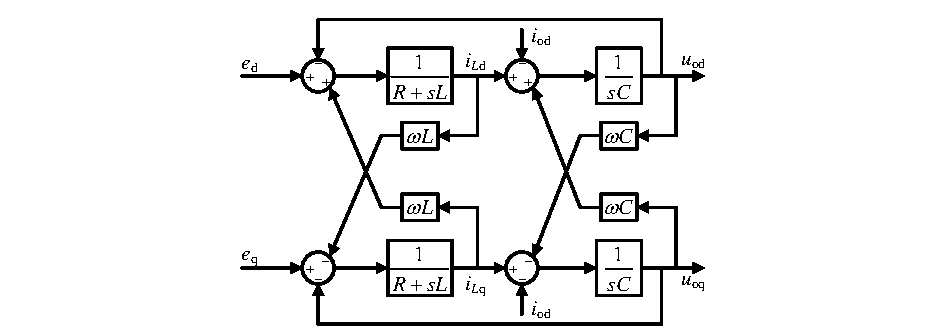
\includegraphics[width=\textwidth]{chapter3/VSI/两相同步旋转坐标系中三相VSI模型结构图.pdf}
	\caption{两相同步旋转dq坐标系中三相VSI模型结构图}
	\label{fig:两相同步旋转dq坐标系中三相VSI模型结构图}
\end{figure}

\section{岸侧变流器系统控制策略}

电压电流瞬时值双闭环控制的系统框图,它的原理为:采样岸电电源的输出电压U0,经过信号调理获得电压反馈信号Vfed,
并和电压给定值Vref相比较得到偏差信号ev。然后送入电压调节器,它的输出值即是电流内环反馈的参考
值Iref,再和电流反馈值If相比较获得误差信号ei。最后经过电流调节器得到控制信号Vc并输出给DSP进行运算处理,
从而对SPWM驱动波形进行调制。

电流内环,电压外环双闭环控制策略。

\begin{figure}[!htp]
	\centering
	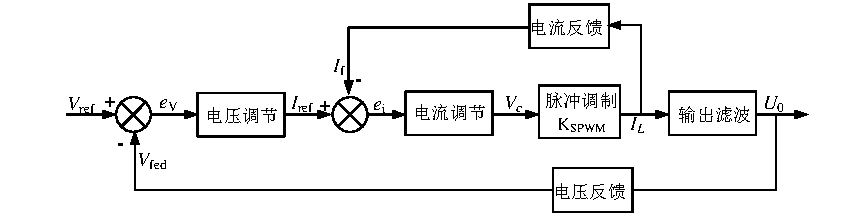
\includegraphics[width=\textwidth]{chapter3/电压电流双闭环控制.pdf}
	\caption{压电流双闭环控制}
	\label{fig:压电流双闭环控制}
\end{figure}

\subsection{变流器整流侧控制方法}

\begin{equation}
	\begin{pmatrix}
		e_d \\ eq
	\end{pmatrix}=
	\begin{pmatrix}
		Lp+R & -\omega L \\ 
		\omega L & Lp+R 
	\end{pmatrix}
	\begin{pmatrix}
		i_d \\ i_q
	\end{pmatrix}+
	\begin{pmatrix}
		u_d \\ u_q
	\end{pmatrix}
\end{equation}

\begin{equation}
	\frac{3}{2}(u_di_d+u_qi_q)=u_{dc}i_{dc}
\end{equation}

\begin{equation}
	\begin{cases}
		u_d = - \left( K_{iP}+\frac{K_{iI}}{s} \right) (i_{d}^{*}-i_d) +\omega Li_q+e_d \\
		u_q = - \left( K_{iP}+\frac{K_{iI}}{s} \right) (i_{q}^{*}-i_q) +\omega Li_d+e_q	
	\end{cases}
\end{equation}

\begin{equation}
	L p\begin{pmatrix}
		i_{\mathrm{d}} \\
		i_{\mathrm{q}}
		\end{pmatrix}=
		\begin{pmatrix}
		-R+K_{i \mathrm{P}}+\frac{K_{i \mathrm{I}}}{s} & 0 \\
		0 & -R+K_{i \mathrm{P}}+\frac{K_{i \mathrm{I}}}{s}
		\end{pmatrix}
		\begin{pmatrix}
		i_{\mathrm{d}} \\
		i_{\mathrm{q}}
		\end{pmatrix}-
		\left(K_{\mathrm{iP}}+\frac{K_{i \mathrm{I}}}{s}\right)
		\begin{pmatrix}
		i_{\mathrm{d}}^{*} \\
		i_{\mathrm{q}}^{*}
		\end{pmatrix}
\end{equation}

\begin{figure}[!htp]
	\centering
	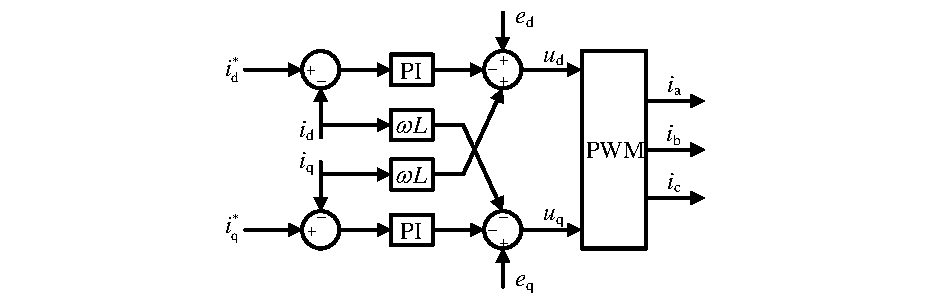
\includegraphics[width=0.9\textwidth]{chapter3/VSR/三相VSR电流内环解耦控制结构.pdf}
	\caption{三相VSR电流内环解耦控制结构}
	\label{fig:三相VSR电流内环解耦控制结构}
\end{figure}

\begin{figure}[!htp]
	\centering
	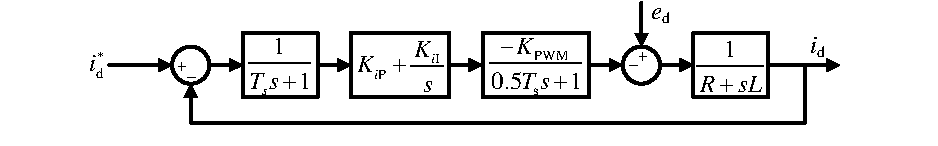
\includegraphics[width=\textwidth]{chapter3/VSR/id电流内环结构.pdf}
	\caption{id电流内环结构}
	\label{fig:id电流内环结构}
\end{figure}

\begin{figure}[!htp]
	\centering
	
\includegraphics[width=\textwidth]{chapter3/VSR/无ed扰动时的id电流内环结构.pdf}
	\caption{无ed扰动时的id电流内环结构}
	\label{fig:无ed扰动时的id电流内环结构}
\end{figure}

\begin{figure}[!htp]
	\centering
	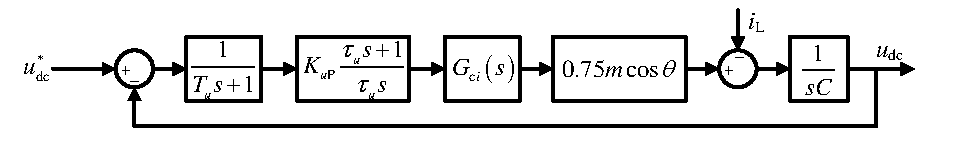
\includegraphics[width=\textwidth]{chapter3/VSR/三相VSR电压外环控制结构.pdf}
	\caption{三相VSR电压外环控制结构}
	\label{fig:三相VSR电压外环控制结构}
\end{figure}

\begin{figure}[!htp]
	\centering
	
\includegraphics[width=\textwidth]{chapter3/VSR/三相VSR电压外环简化结构.pdf}
	\caption{三相VSR电压外环简化结构}
	\label{fig:三相VSR电压外环简化结构}
\end{figure}

\subsection{变流器逆变侧控制方法}

电流内环,电压外环双闭环控制策略。

\begin{figure}[!htp]
	\centering
	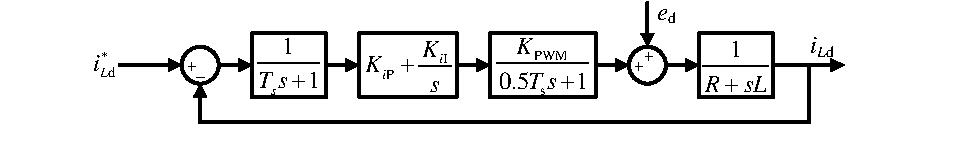
\includegraphics[width=\textwidth]{chapter3/VSI/iLd电流内环结构.pdf}
	\caption{iLd电流内环结构}
	\label{fig:iLd电流内环结构}
\end{figure}

\begin{figure}[!htp]
	\centering
	
\includegraphics[width=\textwidth]{chapter3/VSI/无ed扰动时的iLd电流内环结构.pdf}
	\caption{无ed扰动时的iLd电流内环结构}
	\label{fig:无ed扰动时的iLd电流内环结构}
\end{figure}

\begin{figure}[!htp]
	\centering
	
\includegraphics[width=\textwidth]{chapter3/VSI/Uod电压外环结构.pdf}
	\caption{Uod电压外环结构}
	\label{fig:Uod电压外环结构}
\end{figure}

\begin{figure}[!htp]
	\centering
	
\includegraphics[width=\textwidth]{chapter3/VSI/Uod电压外环简化结构.pdf}
	\caption{Uod电压外环简化结构}
	\label{fig:Uod电压外环简化结构}
\end{figure}

搭建如图\ref{fig:低压岸电系统仿真示意图}所示的岸电仿真模型。

\begin{figure}[!htp]
	\centering
	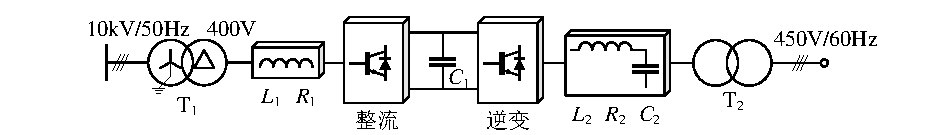
\includegraphics[width=\textwidth]{chapter3/低压岸电换流系统仿真结构示意图.pdf}
	\caption{一种低压岸电系统仿真示意图}
	\label{fig:低压岸电系统仿真示意图}
\end{figure}

\section{系统压降解决方案}

岸基电源输出至接线箱的压降主要有两部分: 输出隔离变压器、输出电缆。

\subsection{隔离变压器的压降问题}

在不同的负载下,隔离变压器压降不同,负载越重,压降越大,针对这一部分问题,解决方案有两种:

方案一: 变频电源对隔离变压器输出侧电压进行采集,将信号传输至变频主控系统,由主控系统进行闭环控制,
稳定控制隔离变压器输出侧电压稳定,此方案控制相对更加精准。

方案二: 根据隔离变压器的阻抗值,将阻抗值输入变频主控算法中,由变频对此压降进行补偿,此方案相对简单。

\subsection{输出电缆的压降问题}

根据不同长度的输出电缆,其压降不同,但总体压降不多,针对此部分压降,可采用电压微调的方式进行,电压微调可通过触摸屏修改。


\section{船舶岸电供电并网切换}
船岸电力的电网连接是在船的柴油发电机和岸上电源之间。并网需要满足四个条件:船舶发电机的相序、幅值、相位、频率
必须与岸电一致。保持相同的相序尤为重要。影响瞬时电压差的三个因素是频率差、相位差和电压差。船岸自动准同步并网
的四个条件如下:
(1)船舶电源的相序必须等于岸上电源的相序;
(2)船舶电源的电压幅值必须等于岸上电源的电压幅值;
(3)船舶电源的频率必须等于岸上电源的频率;
(4)船舶电源的相位必须等于岸上电源的相位。
这些条件在理想情况下得到满足。事实上,相位、频率和振幅不可能同时完全一致。但只要船电和岸电的相位、频率、幅度差
在一定值内,涌流就在系统可接受的范围内,所以可以进行船岸并网。

船舶岸电系统具备船电、岸电快速切换连接技术,通过船上同期装置,与岸电电源实现热并网,保证供电安全
可靠。船舶 岸电 系统接到岸电并网指令后,自动并车装置进行相序检测跟踪,在相序一致的情况 下,采集岸电电源及传
播辅机电源的电压、频率和相角差的信息,并计算判断是否满足以下并车条件:辅机与岸电的频率、相序及 电压幅值保持
一致,并且在并车的瞬间保证船舶辅机与岸电电源的输出电压相角同步。之后 完成并车并实现自动无缝负荷转移。根据船舶岸电
系统不同的供电连接方式,将岸电电源与船舶发电机的切换方式主要分为断电方式和无缝切换方式2种\cite{SP10}。
1)断电方式:当船舶靠港停泊时,需要首先使船舶上所有的用电设备关闭,并使船舶发电机停止工作,然后连接船舶岸电
系统,最后重新启动船舶的用电设备,实现船舶发电机与岸电电源之间的切换;当船舶离港时,按照相反的顺序操作。
2)同步并车方式:也被称为无缝切换方式,切换过程中不需要关闭 船上所有设备。同步并车方式不会影响船舶上用电设备
的正常运行,对船舶上的重要用电设备具有重大意义。无缝切换也是船舶岸电连接技术的发展趋势,对于岸电电源的推广
意义重大。船舶岸电自动并车技术需要保证船舶发电机与岸电电源的电压幅值和频率保持一致,并在并车的瞬间保证船舶发
电机与岸电电 源的输出电压相角同步。如果两路电源不同步就进行切换会造成严重的后果。如果在切换时刻一个电源电压波
形在波峰,另外一个位于波谷,切换过程中将会产生很大的冲击电流。虽然切换装置可能能承受该冲击电流,但严重时可能
会导致用电设备和高压静止频率变换器的自动保护装置动作。

岸电与船舶辅机并网,船舶保证不停电,实现无缝切换方式,变频电源具有主动切换与被动切换两种方式,具体实现如下:

\subsection{主动并网切换}

变频电源仅作为整个电网切换的主体变频,根据采集到的船上辅机发电机发出电源的信息,包括电压及电流。电压信号主要
用于变频输出电压的标准,变频输出锁频锁相,使输出电源的相位、频率、幅值、相序等与船上完全一致。

电流信息主要作用是让变频控制器获得此时发电机的输出功率,进行负载转移,变频控制器可控制输出,使输出功率逐渐增
大,直至将发电机所带负载完全转移至变频电源供电。

主动切换方式目前有少部分应用,其优点是可以做到整个切换过程的智能化,如一键切换,中间所有过程可自动全部完成。
缺点是需要船方的配合进行改造,否则无法知道发电机的电压、电流等信息,系统不具通用性。

\subsection{被动并网切换}

变频电源仅作为恒频稳压的电源,按照要求输出电压及频率,所有的电网之间的切换均依靠船上的同期柜,具体步骤如下:

变频根据命令要求输出电压 /频率,电源通过输出滤波、隔离变、接口箱、船上进线柜,直接送至船载的变频电源并网柜,
并网柜根据采集到的信息,显示电源的相序、频率、幅值、相位等信息,自动判断是否具备并网条件,通过调整发电机的发
电信息,直至具备并网条件后将变频电源接入; 成功并网后,发电机减小输出功率,负载自动逐渐转移至岸用电源供电,切
换完成后,发电机退出工作。

被动切换是目前比较流行、采用最多的方案,因为其具有简单、通用等特点,且可以实现单个电源同时给多条船只供电的情
况; 但缺点是目前船上与岸基电源之间除了安全联锁信号外,没有其他信号交互,自动化程度低,主要原因是岸电电源与船
上之间的通信协议还未形成国际标准。

\section{逆功率处理方案}

\subsection{逆功率产生机理}

岸用电源逆功率产生的机理如图所示。

两个电压源同时给负载供电时,由于并网运行时的相位、频率和幅值之差导致的逆功率。下面从矢量图分析几种逆功率产生
的机理,V1 为岸用电源,V2 为发电机电源。

V→1超前V→2,V→1与i→s夹角θ小于90°,不会出现逆功率情况,如图所示。

\subsection{逆功率的处理}

(1) 检测到逆功率状态时,变频电源主动调节输出频率及输出相位,使V→1与i→s夹角小于 90°,通过软件算法从根本
上解决逆功率问题,主动抑制逆功率的产生;

(2) 采用四象限变频器,当产生逆功时,通过回馈到电网的方式来解决;

(3) 制动电阻吸收方式,当产生逆功时,通过制动电阻来吸收产生的能量。

\subsection{不同控制方案简单对比}

由于逆功率控制仅用于并网瞬间即解列过程,整个过程大概几秒时间,不同的控制方案达到的实际效果不同,
具体对比如表所示。

\section{并网负载转移}

不同船舶的主配电板不一样,并网的切换方式也不一样。日本峙崎和日本 JRCS 的船舶主配电板,并网负载转移方式是按
照负载容量为转移切换的依据,剩余10\% 负载时,柴油发电机退出。

长荣集团船舶、韩国现代船舶主配电板,并网负载转移方式是按照时间为转移的依据,并网后 5 s 船舶柴油发电机退出,
负载直接突加到岸电。

\section{自动电压平衡}

\section{三相输出电压平衡控制技术}

因变频电源的负载有别于变频器的电机类负载,船上单相负载的使用,导致其三相间负载分配不可能绝对的平衡,从而每相之间的压降
可能会有不同。通过三相输电压平衡控制技术,对三相输出电压实行闭环控制。

\section{船岸等电位处理方案}

岸电系统的接地系统相对要重点关注,虽然海水导电,但它存在电阻,船体( “地”) 和岸地因传导电阻造成电位差,有电位
差就会产生电流,威胁人身安全,故无论是低压还是岸电,均要求船岸的“地”保持等电位连接,以降低接触电压,提高安全
用电水平。在岸电连船过程中应注意该等电位连接不应改变船舶配电系统的接地原理。对于船岸之间的等电位连接设计如下:
船岸连接等电位线集成于船岸连接动力电缆中,将船舶外壳、岸电系统外壳、码头电源插座箱箱体与码头电网相连,
如图所示为等电位连接线方案。


\section{本章小结}
	\chapter{船岸连接系统并网与解列分析}

\begin{figure}[!htp]
	\centering
	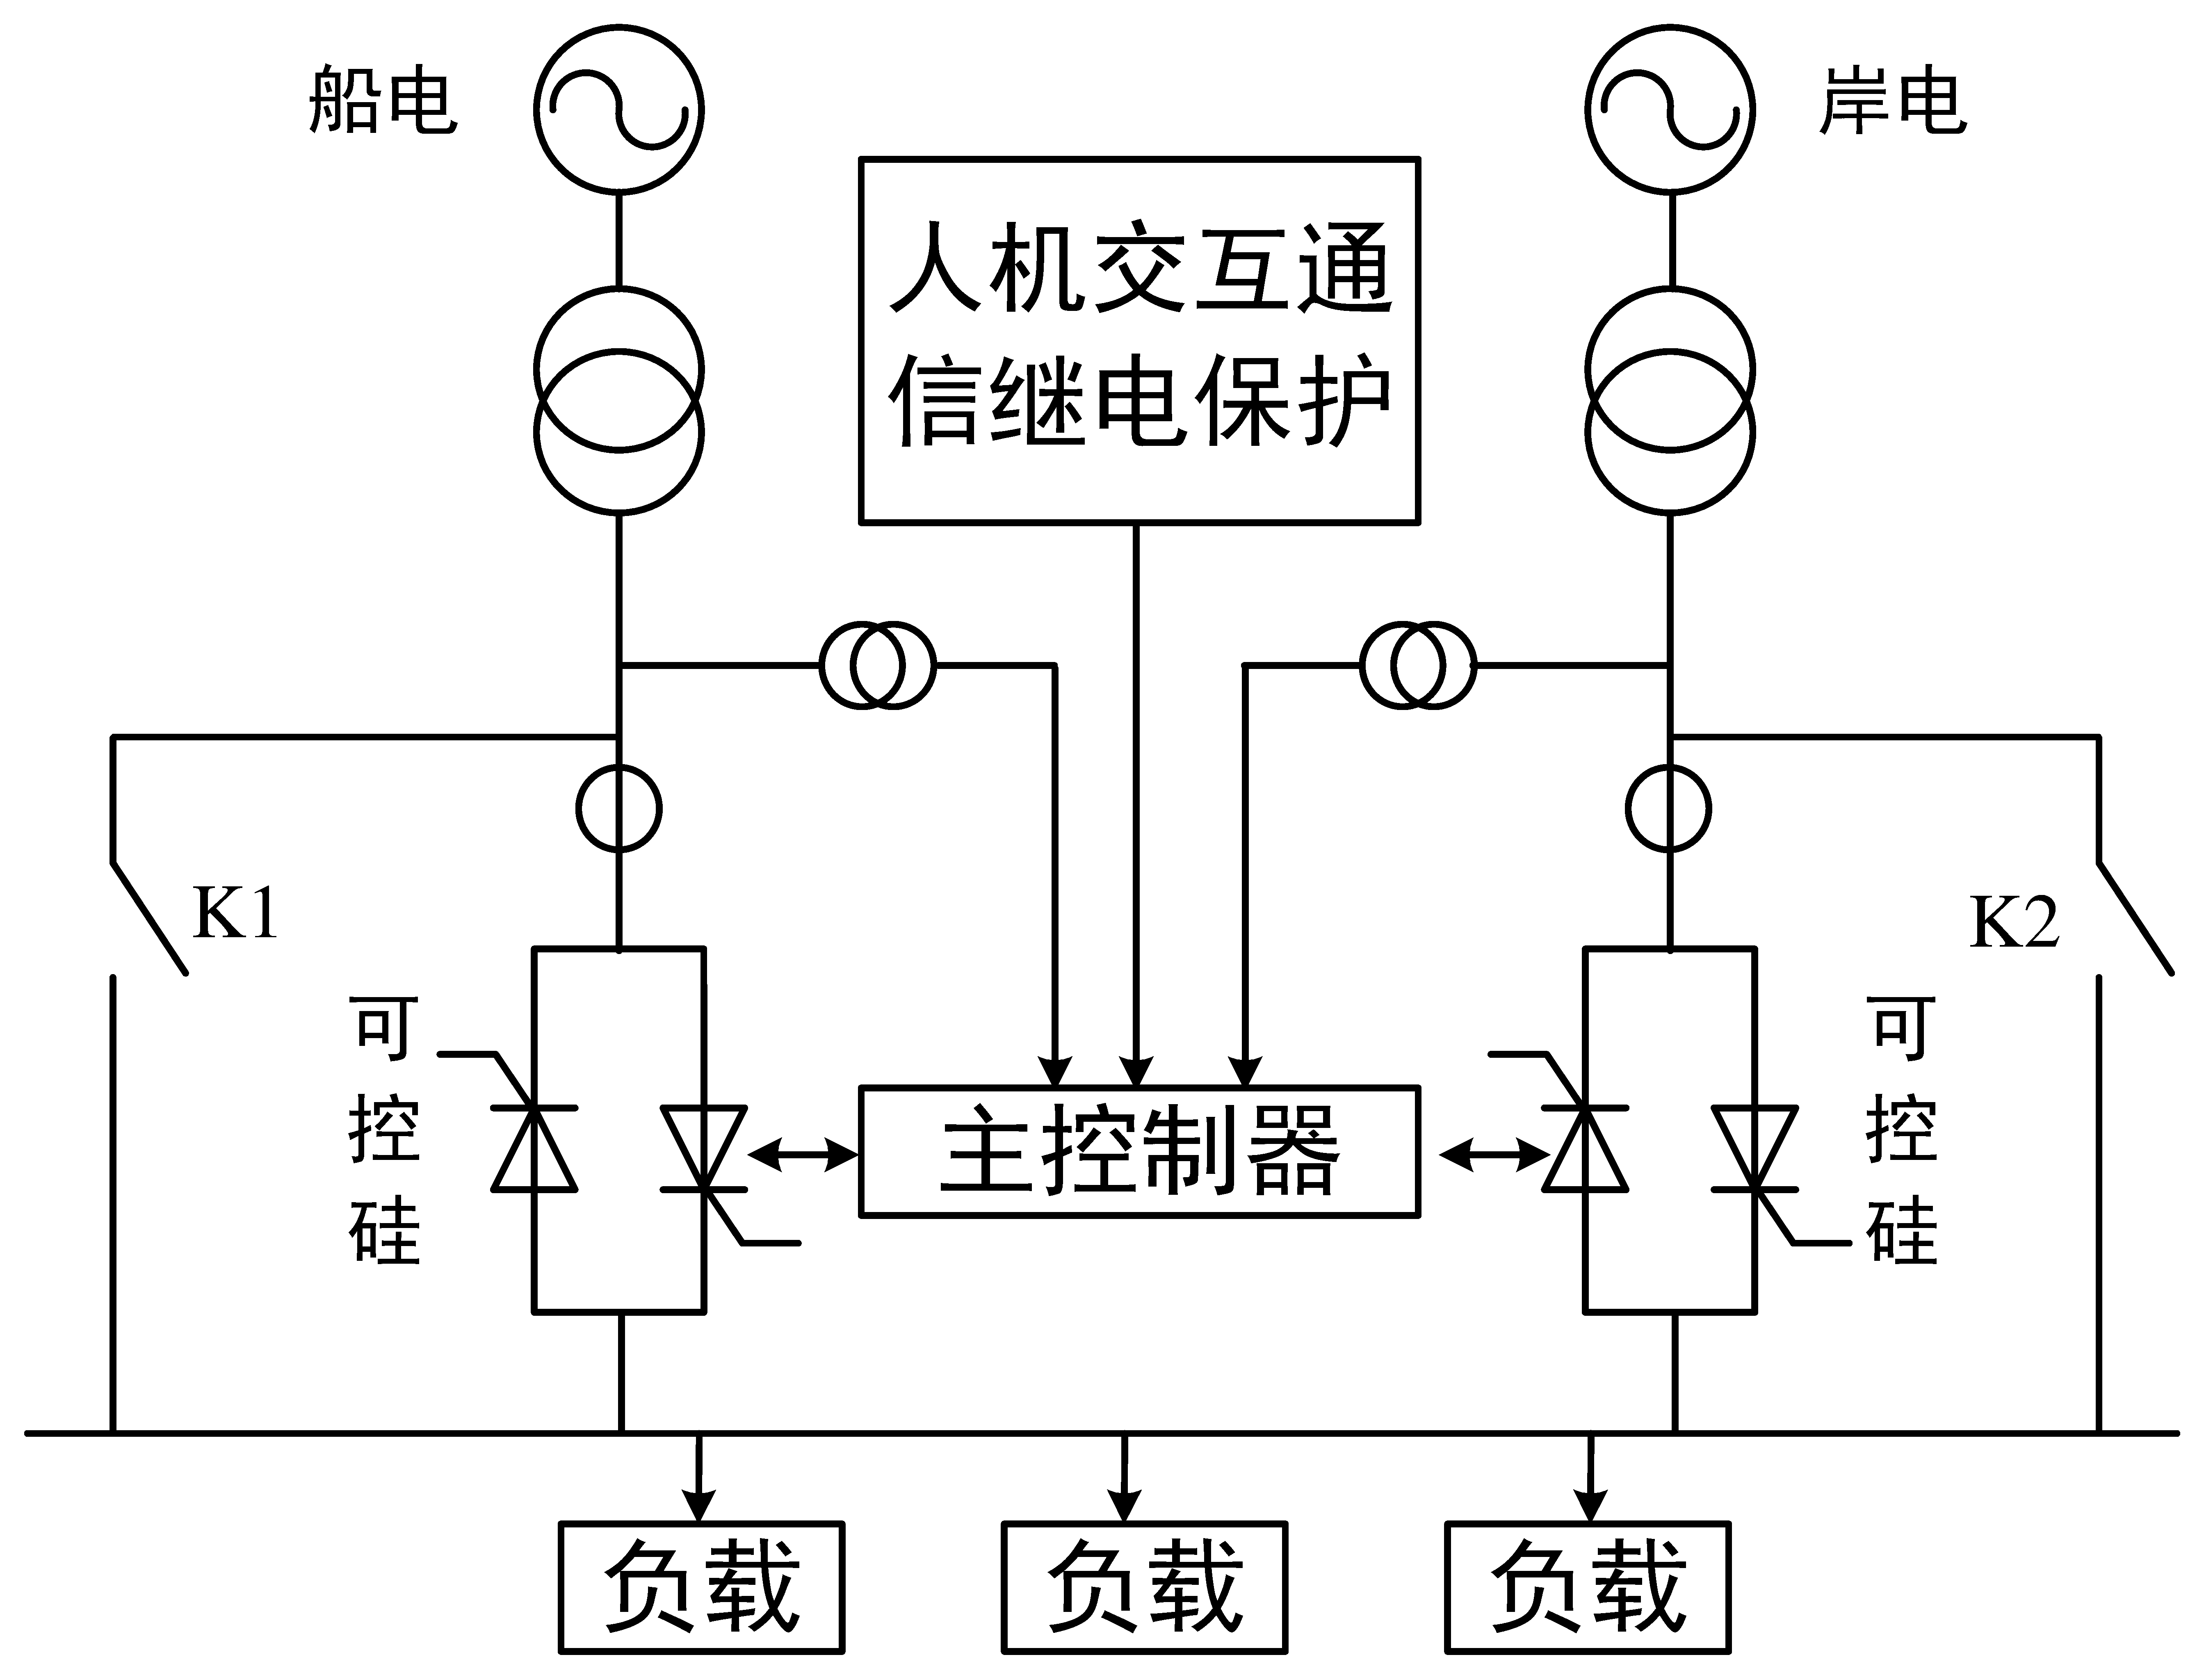
\includegraphics[width=0.5\textwidth]{chapter4/固态开关切换结构图.pdf}
	\caption{固态开关切换结构图}
	\label{fig:固态开关切换结构图}
\end{figure}

\section{船岸连接系统并网与解列条件}

\subsection{岸电并入船舶电网条件}

\subsection{岸电解列船舶电网条件}

\section{船岸连接系统并网与解列过程}

\subsection{岸电并入船舶电网过程}


\begin{figure}[!htp]
	\centering
	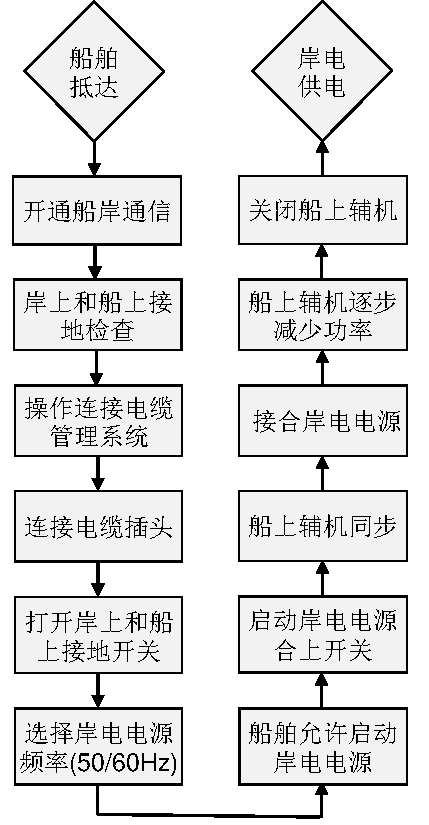
\includegraphics[width=0.45\textwidth]{chapter4/并网过程.pdf}
	\caption{岸电电源并网船舶电网流程图}
	\label{fig:岸电电源并网船舶电网流程图}
\end{figure}


\begin{figure}[!htp]
	\centering
	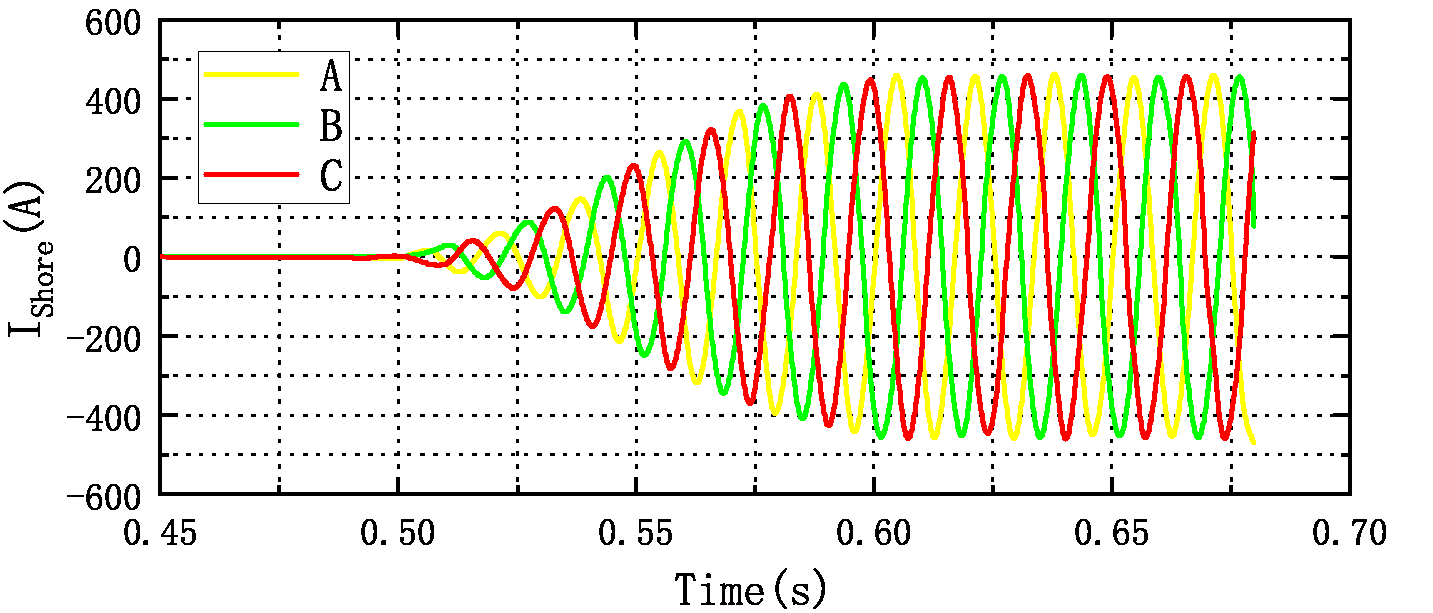
\includegraphics[width=0.9\textwidth]{chapter4/并网/并网过程岸电电流.pdf}
	\caption{船舶岸电并网时电流变化情况}
	\label{fig:船舶岸电并网时电流变化情况}
\end{figure}

\begin{figure}[!htp]
	\centering
	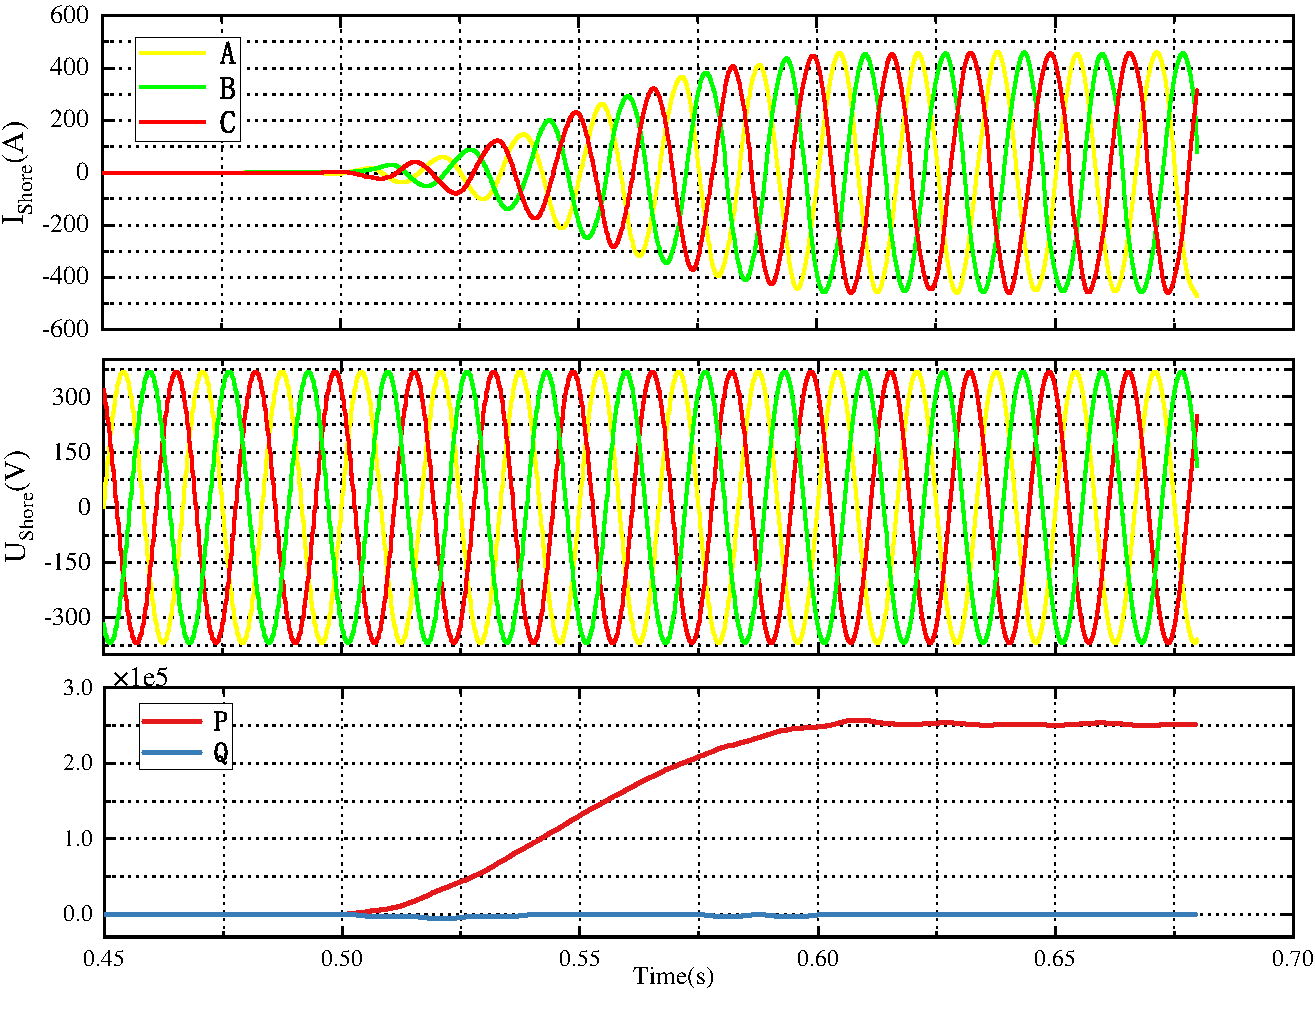
\includegraphics[width=0.9\textwidth]{chapter4/并网/岸电并网情况.pdf}
	\caption{船舶岸电并网情况}
	\label{fig:船舶岸电并网情况}
\end{figure}

\begin{figure}[!htp]
	\centering
	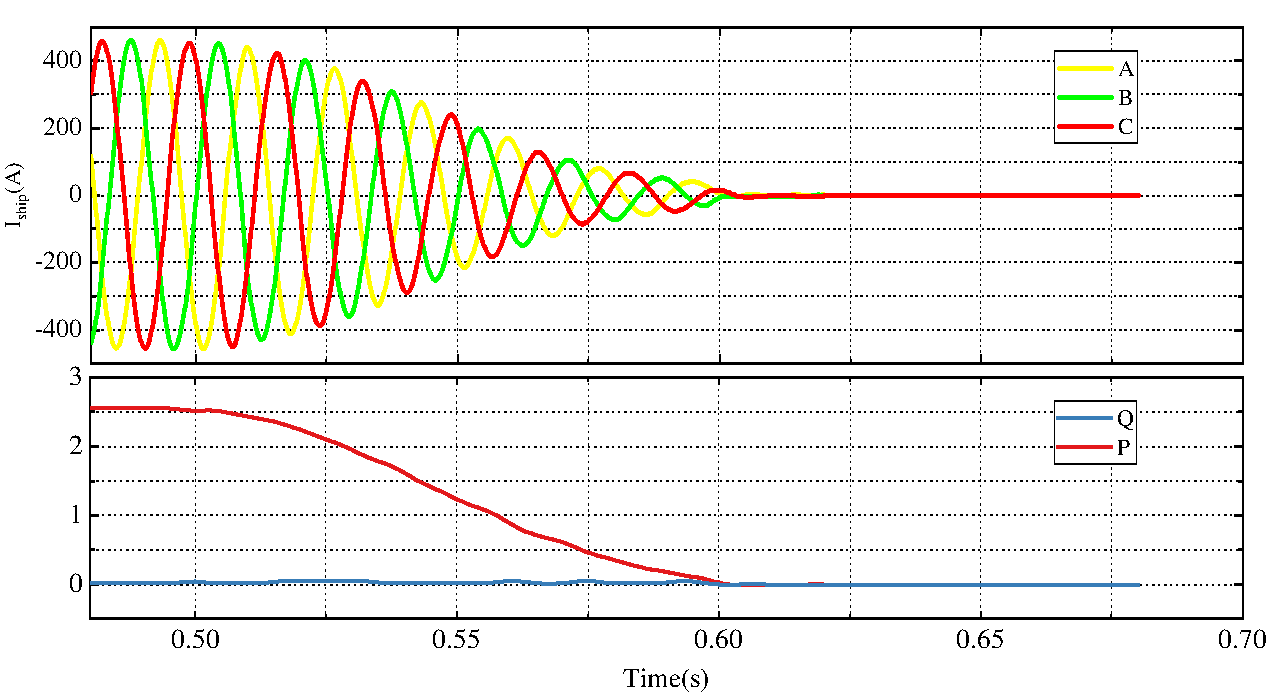
\includegraphics[width=0.9\textwidth]{chapter4/并网/并网船舶发电机情况.pdf}
	\caption{船舶发电机并网情况}
	\label{fig:船舶发电机并网情况}
\end{figure}


\subsection{岸电解列船舶电网过程}

\begin{figure}[!htp]
	\centering
	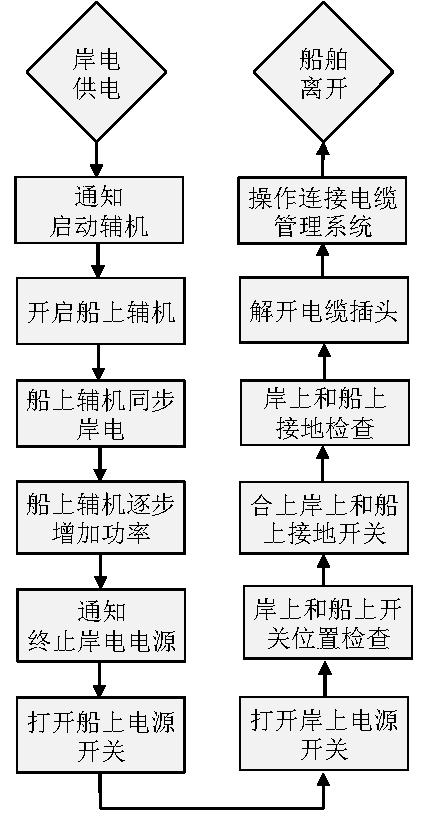
\includegraphics[width=0.45\textwidth]{chapter4/解列过程.pdf}
	\caption{岸电电源解列船舶电网流程图}
	\label{fig:岸电电源解列船舶电网流程图}
\end{figure}

\section{船岸连接系统并网与解列控制方法}

\subsection{基于同步旋转坐标系的锁相环设计}

\subsection{负载转移过程控制与分析}

\begin{table}[!htp]
	\centering
	\caption[电压和频率波动表]{电压和频率波动表\cite{SP7}}
	\label{tab:电压和频率波动表}
	\resizebox{0.9\textwidth}{!}{%
	\begin{tabular}{c}
		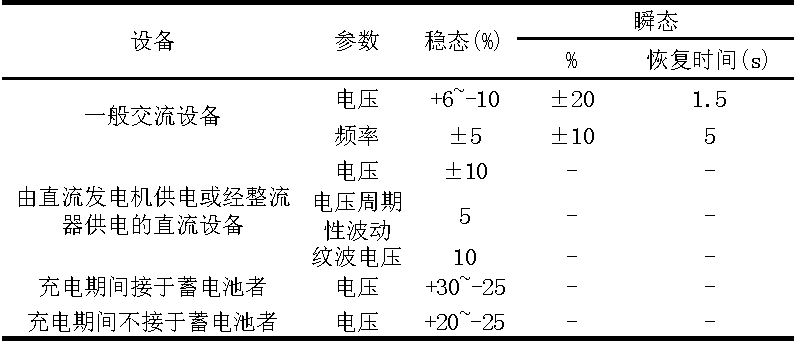
\includegraphics{chapter4/电压和频率波动表.pdf} 
	\end{tabular}
	}
\end{table}

\section{船岸连接系统并网与解列仿真}




\section{本章小结}





	\chapter{船岸连接监控与控制系统设计}

\begin{figure}[!htp]
	\centering
	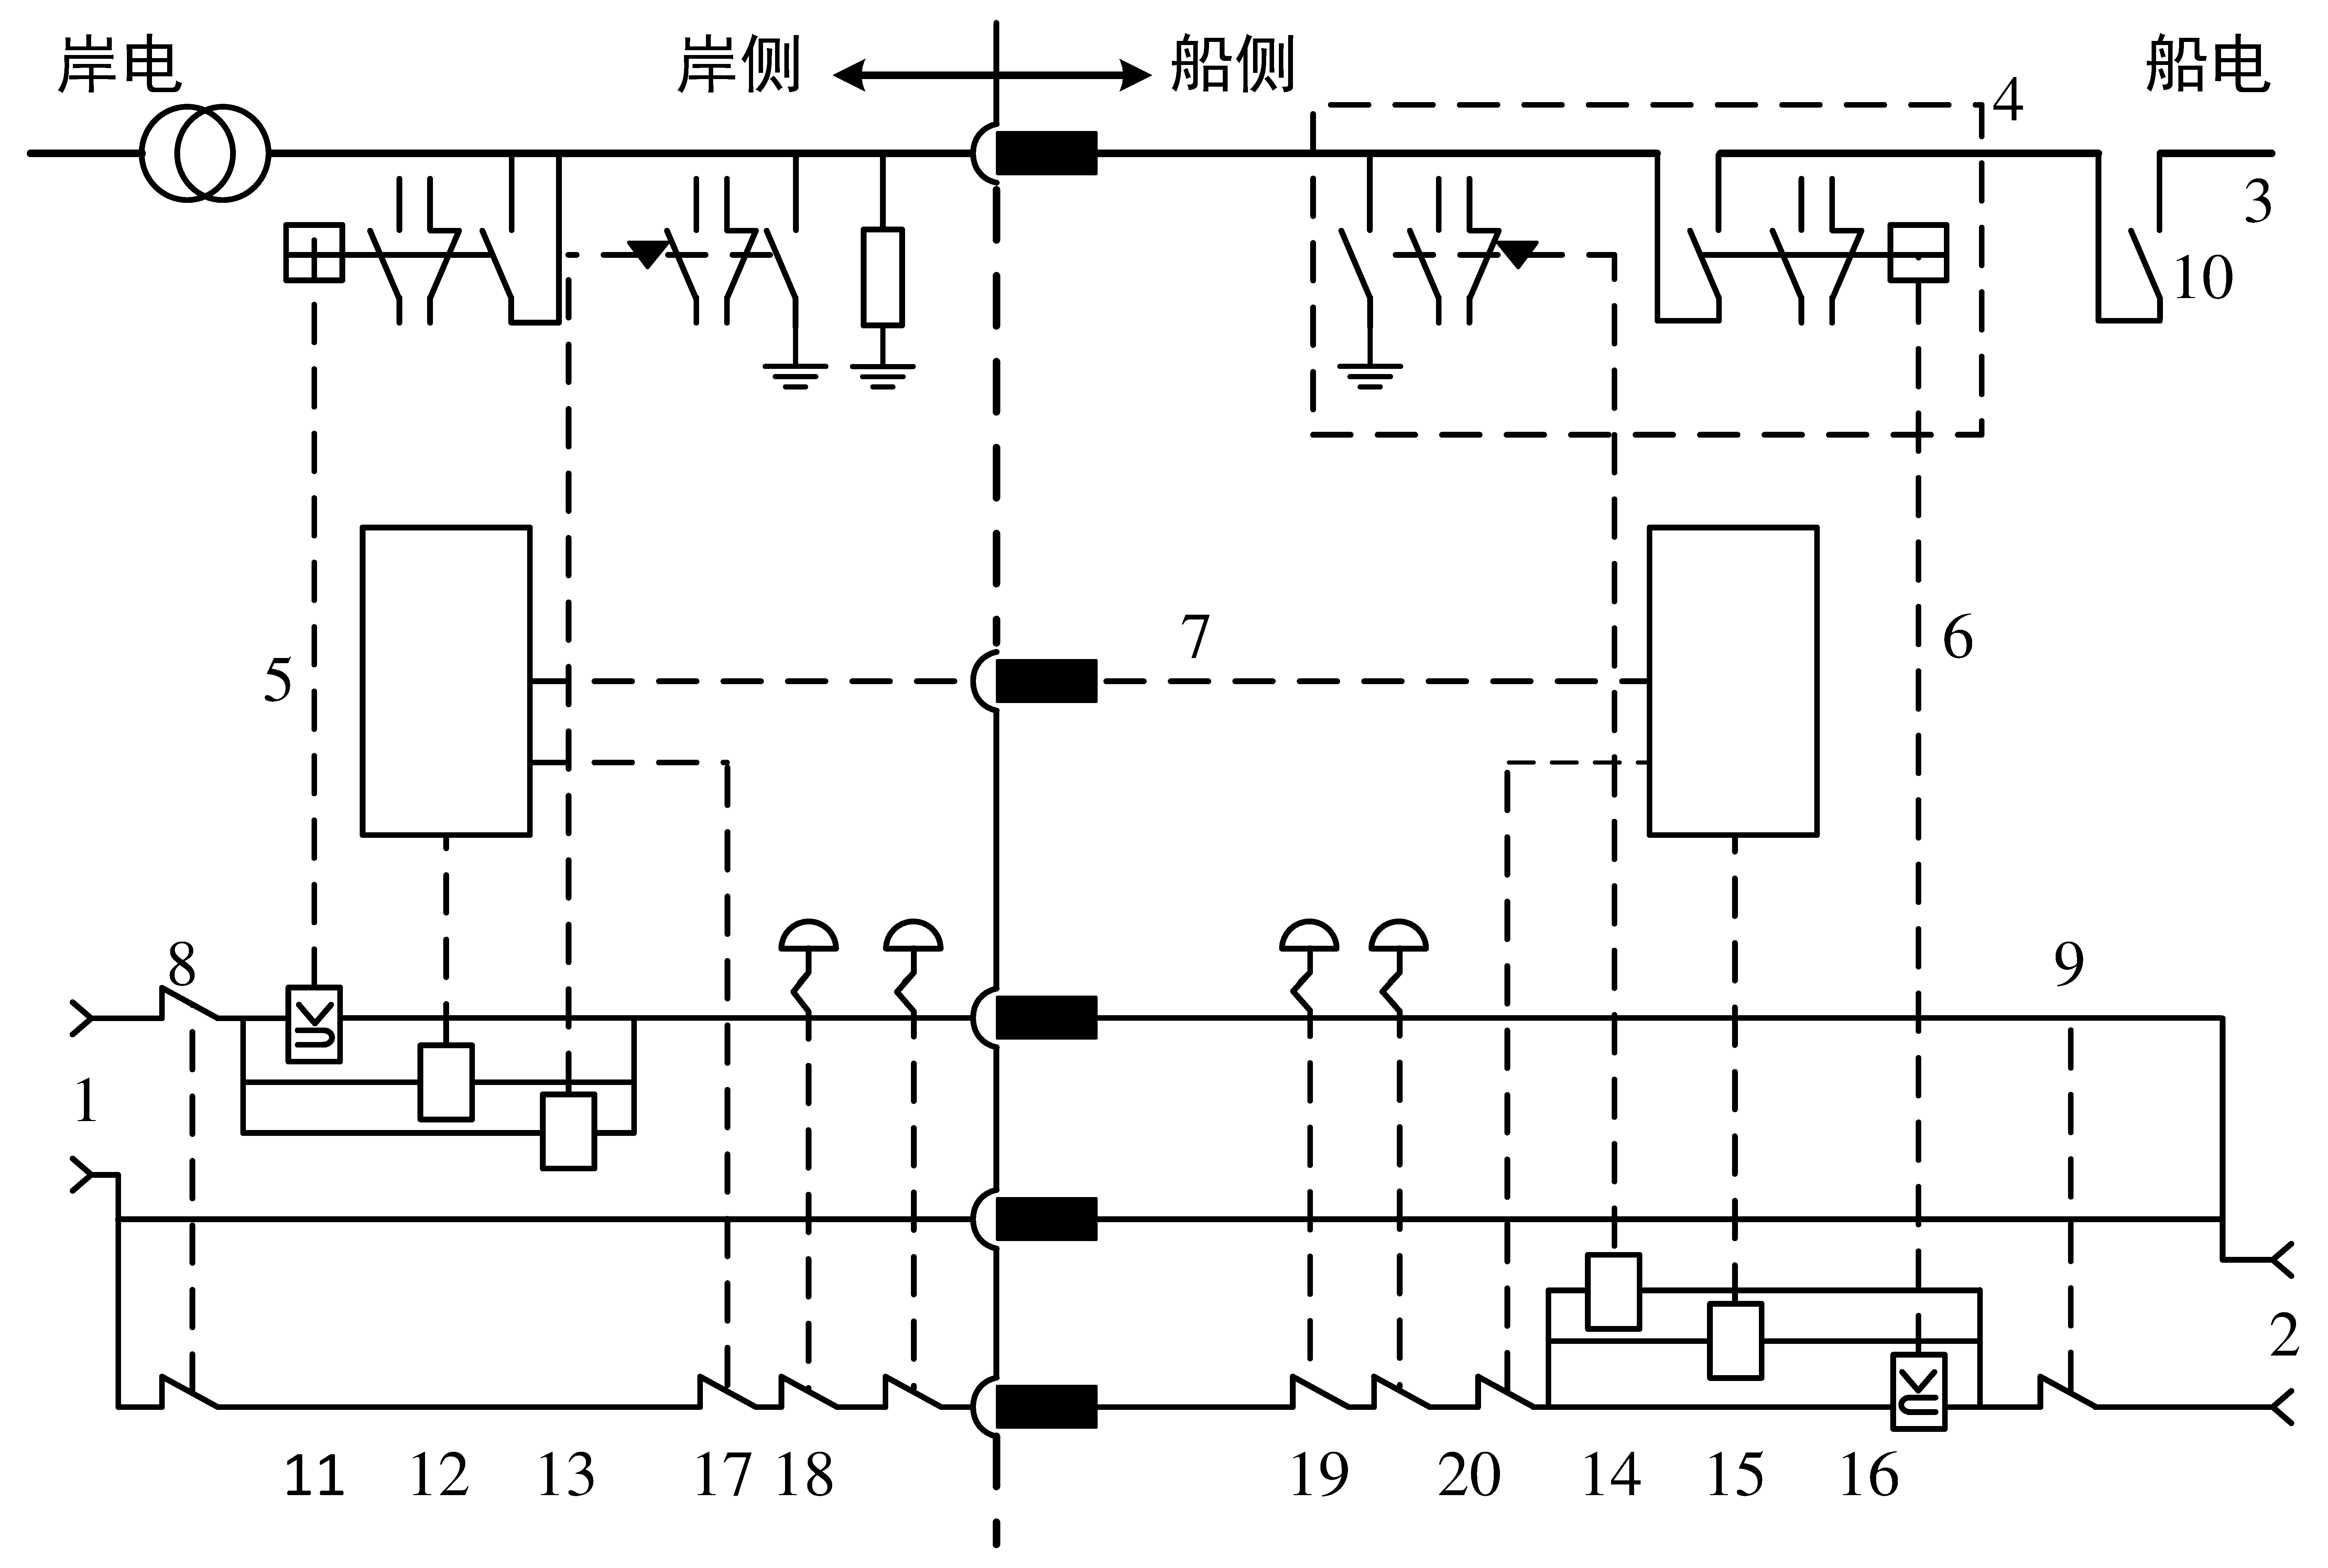
\includegraphics[width=0.8\textwidth]{chapter5/岸电电源控制系统原理图.pdf}
	\caption{岸电电源控制系统原理图}
	\label{fig:岸电电源控制系统原理图}
    {\kaishu \zihao{5}
    \hspace*{\fill} 

    1-岸侧控制电源;2-船侧控制电源;3-船舶电网;4-船电岸电切换柜;

    5-岸电PLC控制器;6-船侧PLC控制器;7-光纤通信;8-岸电保护;

    9-船电保护;10-同步切换开关;11-岸电切换开关;12-岸电保护开关;
    
    13-岸侧接地允许;14-船侧接地允许;15-船侧安全保护;16-船侧切断开关;

    17-船侧接地控制;18-船侧手动接地;19-岸侧控制接地;20-岸侧手动接地;

    }
\end{figure}

\section{第一节}

\subsection{子节点}
	\chapter{总结与展望}

\section{全文总结}

\section{展望}



%不引用但可以显示参考文献方式
\nocite{*}

	% 正文内容
	\chapter{绪论}

这是 \shmtuthesis 的示例文档,基本上覆盖了模板中所有格式的设置。建议大家在使用模板之前,除了阅读《\shmtuthesis\ 使用文档》,这个示例文档也最好能看一看。

\section{二级标题}

\subsection{三级标题}

\subsubsection{四级标题}

\zhlipsum[1-2]

\section{脚注}

上海海事大学的校训 “忠信笃敬” ,通常形容言行举止很忠义,值得别人相信,自己做的事也受到别人的尊敬。\footnote{出自《论语·卫灵公》:“言忠信,行笃敬,虽蛮貊之邦,行矣.言不忠信,行不笃敬,虽州里,行乎哉?”}

\section{字体}
{默认字体——宋体:中国高等航海教育发轫于上海,1909年晚清邮传部上海高等实业学堂(南洋公学)船政科开创了我国高等航海教育的先河。1912年成立吴淞商船学校,1933年更名为吴淞商船专科学校。1959年交通部在沪组建上海海运学院。2004年经教育部批准更名为上海海事大学。为更好地服务上海国际航运中心建设和国家航运事业发展,根据上海市高校布局结构调整规划,2008年上海海事大学主体搬迁临港新城(现上海自贸区临港新片区)。2019年学校成功举行110年校庆系列活动。} 

{宋体——\cs{songti}:\songti 上海海事大学是一所以航运、物流、海洋为特色,具有工学、管理学、经济学、法学、文学、理学和艺术学等学科门类的多科性大学。2008年,上海市人民政府与交通运输部签订协议,共建上海海事大学。}

{黑体——\cs{heiti}:\heiti 学校设有3个博士后科研流动站(交通运输工程、电气工程、管理科学与工程),4个一级学科博士点(交通运输工程、管理科学工程、船舶与海洋工程、电气工程),23个二级学科博士点,16个一级学科硕士学位授权点,60个二级学科硕士学位授权点,12个专业学位授权类别,48个本科专业。拥有12个省部级重点研究基地。现有1个国家重点(培育)学科,1个上海市高峰学科,2个上海市高原学科,9个部市级重点学科,工程学科进入ESI全球前1\%,港航物流学科保持全球领先。5个国家级特色专业,1个国家级综合改革试点专业,7个国家级一流本科专业建设点,6个教育部卓越工程师教育培养计划专业,17个上海市本科教育高地。现有2个国家级实验教学示范中心,2个国家级虚拟仿真实验教学示范中心,5个国家级实践教学示范中心,1个全国示范性工程专业学位研究生联合培养基地。设有水上训练中心,拥有万吨级集装箱教学实习船“育锋”轮,4.8万吨散货教学实习船“育明”轮。}

{楷书——\cs{\kaishu}:\kaishu 在2004年教育部本科教学工作水平评估和2006年教育部英语专业教学评估中获得优秀。2018年,年度科技总经费达到3.7亿元,获一批国家级科研项目及部市级以上科技进步奖。}

{仿宋——\cs{fangsong}:\fangsong 实行校院二级管理体制,现设有商船学院、交通运输学院、经济管理学院(设亚洲邮轮学院)、物流工程学院(设中荷机电工程学院)、法学院、信息工程学院、外国语学院、海洋科学与工程学院、文理学院(设马克思主义学院)、徐悲鸿艺术学院、物流科学与工程研究院、上海高级国际航运学院等二级办学部门。在24000余名学生中,有本科生16500余人,各类在校研究生近6000人,留学生近700名。在1200余名专任教师中,有教授160余名,具有博士学位的教师比例约63\%。学校致力于培养国家航运业所需要的各级各类专门人才,已向全国港航企事业单位及政府部门输送了毕业生逾16万,被誉为“高级航运人才的摇篮”。}

{隶书——\cs{lishu}:\lishu 学校2013年成立中国(上海)自贸区供应链研究院和上海高级国际航运学院。中国(上海)自贸区供应链研究院将自贸区建设与供应链研究有机结合,以提升自贸区产业链建设水平,促进自贸区货物贸易向服务贸易的转型发展,同时推动政府监管职能的转变。上海高级国际航运学院采取国际上先进的商学院运作模式,与全球优秀教育机构资源共享,着力打造国内领先、国际知名的航运金融教育品牌,构筑具有影响力的航运高端人才输出基地。}

{幼园——\cs{youyuan}:\youyuan 2008年,上海市教育委员会、上海市城乡建设和交通委员会、上海海事大学、虹口区人民政府等20多家单位共同发起成立上海国际航运研究中心。中心挂靠上海海事大学,是国际航运业发展的研究和咨询机构,为政府和国内外企业与航运机构等提供决策咨询和信息服务,是上海市教委首批建立的“高校知识服务平台”之一。 2014年,市教委将该平台挂牌为“上海市协同创新中心”。

学校与境外100余所姐妹院校建立了校际交流与合作关系,开展教师交流、合作办学、合作科研、学生交换等。与联合国国际海事组织、波罗的海国际航运公会、挪威船级社等国际知名航运组织/机构建立了密切联系。自2010年起开设“国际班”,邀请美国、韩国、波兰、俄罗斯、德国等国家航海院校的学生来校学习“航海技术”“航运管理”等专业。2011年,经教育部批准,学校与加纳中西非地区海事大学合作举办“物流管理”本科教育项目,并开始在非洲招生,这是上海市地方高校第一个颁发中国高校本科文凭的海外办学项目。2012年,学校获教育部批准正式成为“接受中国政府奖学金来华留学生院校”。}

\section{字号}

\begin{itemize}
	\item {\zihao{0} 初号:\cs{zihao{0}}}
	\item {\zihao{-0} 小初:\cs{zihao{-0}}}
	\item {\zihao{1} 一号:\cs{zihao{1}}}
	\item {\zihao{-1} 小一号:\cs{zihao{-1}}}
	\item {\zihao{2} 二号:\cs{zihao{2}}}
	\item {\zihao{-2} 小二号:\cs{zihao{-2}}}
	\item {\zihao{3} 三号:\cs{zihao{3}}}
	\item {\zihao{-3} 小三号:\cs{zihao{-3}}}
	\item {\zihao{4} 四号:\cs{zihao{4}}}
	\item {\zihao{-4} 小四号:\cs{zihao{-4}}}
	\item {\zihao{5} 五号:\cs{zihao{5}}}
	\item {\zihao{-5} 小五号:\cs{zihao{-5}}}
	\item {\zihao{6} 六号:\cs{zihao{6}}}
	\item {\zihao{-6} 小六号:\cs{zihao{-6}}}
	\item {\zihao{7} 七号:\cs{zihao{7}}}
	\item {\zihao{8} 八号:\cs{zihao{8}}}
\end{itemize}

	\chapter{浮动体}

\section{插图}

插图功能是利用 \TeX\ 的特定编译程序提供的机制实现的,不同的编译程序支持不同的图形方式。有的同学可能听说“\LaTeX\ 只支持 EPS”,事实上这种说法是不准确的。\XeTeX 可以很方便地插入 EPS、PDF、PNG、JPEG、JPG 格式的图片。

一般图形都是处在浮动环境中。之所以称为浮动是指最终排版效果图形的位置不一定与源文件中的位置对应,这也是刚使用 \LaTeX\ 同学可能遇到的问题。如果要强制固定浮动图形的位置,请使用 \pkg{float} 宏包,它提供了 \texttt{[H]} 参数。

\subsection{单个图形}

图要有图注,并置于图的编号之后,图的编号和图注应置于图下方的居中位置。引用图应在图题右上角标出文献来源。当插图中组成部件由数字或字母等编号表示时,可在插图下方添加图注进行说明,如图~\ref{fig:shmtu-school-motto} 所示。一般来说,研究生图注与表注一般要求中英文对照。但是由于上海海事大学没有明确要求,故推荐仅使用中文图注。若有需要添加双语图注,用法如图~\ref{fig:shmtu-school-motto-2}所示。

\begin{figure}[!htp]
	\centering
	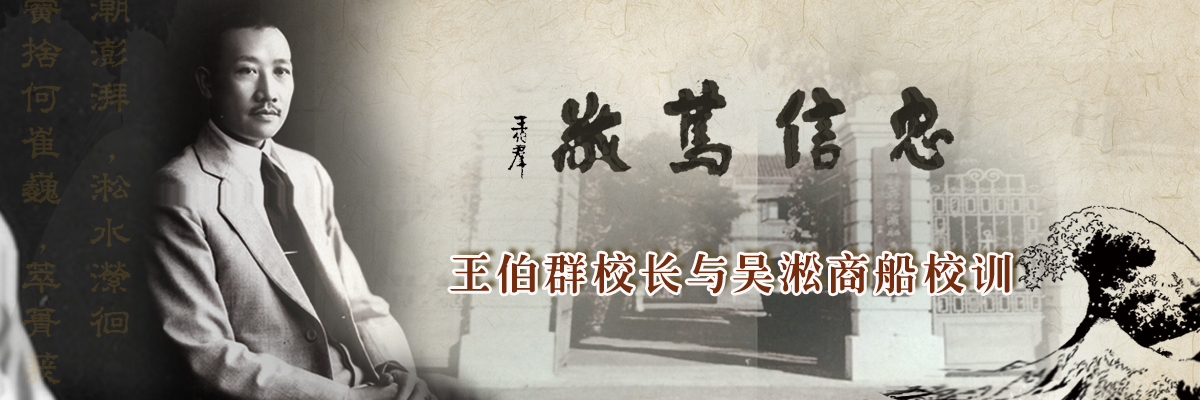
\includegraphics[width=10cm]{shmtu-school-motto}
	\caption{王伯群校长与吴淞商船校训}
	\label{fig:shmtu-school-motto}
\end{figure}

\begin{figure}[!htp]
	\centering
	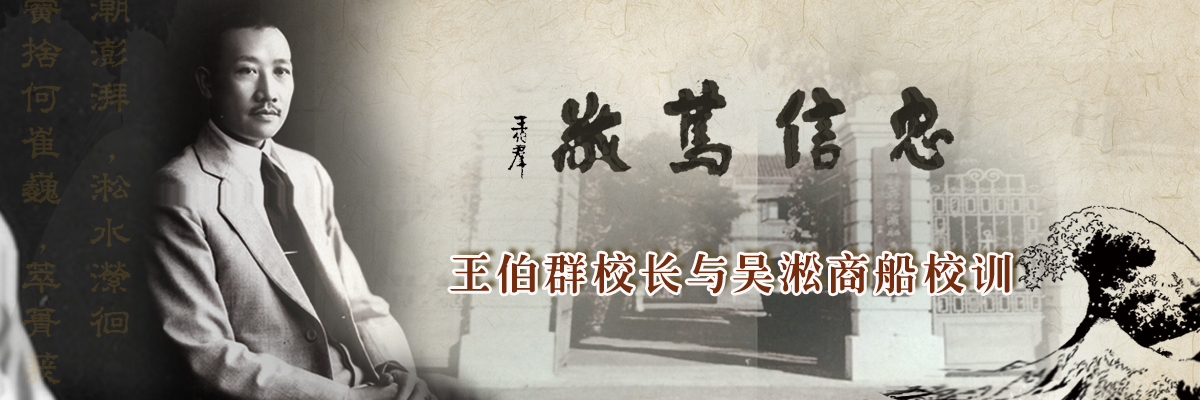
\includegraphics[width=10cm]{shmtu-school-motto}
	\bicaption{王伯群校长与吴淞商船校训}{President Wang Boqun and the school motto of WuSong Merchant Shipping}
	\label{fig:shmtu-school-motto-2}
\end{figure}

\subsection{多个图形}

简单插入多个图形的例子如图~\ref{fig:parallel-1} 所示。这两个水平并列放置的子图共用一个图形计数器,没有各自的子图题。

\begin{figure}[!htp]
  \centering
  
\includegraphics[height=2cm]{images/shmtu-badge}
  \hspace{1cm}
  
\includegraphics[height=2cm]{images/shmtu-badge}
  \caption{上海海事大学校徽}
  \label{fig:parallel-1}
\end{figure}

如果多个图形相互独立,并不共用一个图形计数器,那么用 \cs{minipage} 或者\cs{parbox} 就可以,如图~\ref{fig:parallel-2-1} 与图~\ref{fig:parallel-2-2}。

\begin{figure}[!htp]
  \begin{minipage}{0.48\textwidth}
  	\centering
    
\includegraphics[height=1.5cm]{images/shmtu-badge.jpg}
    \caption{并排第一个图}
    \label{fig:parallel-2-1}
  \end{minipage}
  \hfill
  \begin{minipage}{0.48\textwidth}
    \centering
    
\includegraphics[height=1.5cm]{images/shmtu-badge.jpg}
    \caption{并排第二个图}
    \label{fig:parallel-2-2}
  \end{minipage}
\end{figure}

如果要为共用一个计数器的多个子图添加子图注,那么使用\cs{subcaptionbox}(双语图注使用\cs{bisubcaptionbox})并排子图,子图注置于子图之下,子图号用 (a)、(b)、(c)等表示。如图~\ref{fig:subcaptionbox}、图~\ref{fig:subcaptionbox-a}、图~\ref{fig:subcaptionbox-b}、图~\ref{fig:subcaptionbox-c}所示。

\begin{figure}[!htp]
  \subcaptionbox{上海海事大学校徽\label{fig:subcaptionbox-a}}%
	[0.5\textwidth]{%
	  
\includegraphics[height=1.5cm]{images/shmtu-badge}
	}
  \hfill
  \subcaptionbox{上海海事大学校名\label{fig:subcaptionbox-b}}%
    [0.5\textwidth]{%
	  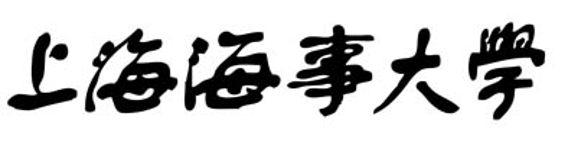
\includegraphics[width=0.5\textwidth]{images/shmtu-name}
	}
  \hfill
  \subcaptionbox{上海海事大学校徽\label{fig:subcaptionbox-c}}%
    [\textwidth]{%
	  
\includegraphics[height=1.5cm]{images/shmtu-badge}
  }
  \caption{共用一个计数器的多个子图图注}
  \label{fig:subcaptionbox}
\end{figure}

\section{表格}

\subsection{基本表格}

编排表格应简单明了,表达一致,明晰易懂,表文呼应、内容一致。表注置于表上,研究生学位论文可以用中、英文两种文字居中排写,中文在上,也可以只用中文。

表格的编排采用国际通行的三线表\footnote{三线表,以其形式简洁、功能分明、阅读方便而在科技论文中被推荐使用。三线表通常只有 3 条线,即顶线、底线和栏目线,没有竖线。}。三线表可以使用 \pkg{booktabs} 提供的 \cs{toprule}、\cs{midrule} 和 \cs{bottomrule}。它们与 \pkg{longtable} 能很好的配合使用。

\begin{table}[!htp]
  \centering
  \caption[一个标准的三线表]{一个标准的三线表\footnotemark}
  \label{tab:firstone}
  \begin{tabular}{llr}  
    \toprule
    \multicolumn{2}{c}{Item} \\
    \cmidrule(r){1-2}
    Animal    & Description & Price (\$) \\
    \midrule
    Gnat      & per gram    & 13.65      \\
              &    each     & 0.01       \\
    Gnu       & stuffed     & 92.50      \\
    Emu       & stuffed     & 33.33      \\
    Armadillo & frozen      & 8.99       \\
    \bottomrule
  \end{tabular}
\end{table}
\footnotetext{这个例子来自
  \href{https://mirrors.sjtug.sjtu.edu.cn/ctan/macros/latex/contrib/booktabs/booktabs.pdf}%
  {《Publication quality tables in LaTeX》}(\pkg{booktabs} 宏包的文档)。这也是
  一个在表格中使用脚注的例子,请留意与 \pkg{threeparttable} 实现的效果有何不
  同。}
  
\subsection{复杂表格}

我们经常会在表格下方标注数据来源,或者对表格里面的条目进行解释。可以用\pkg{threeparttable} 实现带有脚注的表格,如表~\ref{tab:footnote}。

\begin{table}[!htpb]
  \bicaption{一个带有脚注的表格的例子}{A Table with footnotes}
  \label{tab:footnote}
  \centering
  \begin{threeparttable}[b]
     \begin{tabular}{ccd{4}cccc}
      \toprule
      \multirow{2}*{total} & \multicolumn{2}{c}{20\tnote{a}} & \multicolumn{2}{c}{40} & \multicolumn{2}{c}{60} \\
      \cmidrule(lr){2-3}\cmidrule(lr){4-5}\cmidrule(lr){6-7}
      & www & \multicolumn{1}{c}{k} & www & k & www & k \\ % 使用说明符 d 的列会自动进入数学模式,使用 \multicolumn 对文字表头做特殊处理
      \midrule
      & $\underset{(2.12)}{4.22}$ & 120.0140\tnote{b} & 333.15 & 0.0411 & 444.99 & 0.1387 \\
      & 168.6123 & 10.86 & 255.37 & 0.0353 & 376.14 & 0.1058 \\
      & 6.761    & 0.007 & 235.37 & 0.0267 & 348.66 & 0.1010 \\
      \bottomrule
    \end{tabular}
    \begin{tablenotes}
      \item [a] the first note.% or \item [a]
      \item [b] the second note.% or \item [b]
    \end{tablenotes}
  \end{threeparttable}
\end{table}

\zhlipsum[1]

如某个表需要转页接排,可以用 \pkg{longtable} 实现。接排时表注省略,表头应重复书写,并在右上方写“续表 xx”,如表~\ref{tab:grid_mlmmh}。

\begin{longtable}[c]{c*{3}{r}}
  \caption[高变网格的可行三元组]{高变网格的可行三元组, MLMMH.}
  \label{tab:grid_mlmmh} \\
  % 表头
  \toprule
  \multicolumn{1}{c}{Time (s)} & \multicolumn{1}{c}{Triple chosen} & \multicolumn{1}{c}{Other feasible triples} \\
  \midrule
  \endfirsthead
	
  % 续表
  \multicolumn{3}{r}{续表~\thetable} \\
  \toprule
  % 续表表头
  \multicolumn{1}{c}{\textbf{Time (s)}} & \multicolumn{1}{c}{\textbf{Triple chosen}} & \multicolumn{1}{c}{\textbf{Other feasible triples}} \\ 
  \midrule
  \endhead

  \midrule
  \multicolumn{3}{r}{续下页} \\
  \endfoot
  
  \bottomrule
  \endlastfoot
  
0 & (1, 11, 13725) & (1, 12, 10980), (1, 13, 8235), (2, 2, 0), (3, 1, 0) \\
2745 & (1, 12, 10980) & (1, 13, 8235), (2, 2, 0), (2, 3, 0), (3, 1, 0) \\
5490 & (1, 12, 13725) & (2, 2, 2745), (2, 3, 0), (3, 1, 0) \\
8235 & (1, 12, 16470) & (1, 13, 13725), (2, 2, 2745), (2, 3, 0), (3, 1, 0) \\
10980 & (1, 12, 16470) & (1, 13, 13725), (2, 2, 2745), (2, 3, 0), (3, 1, 0) \\
13725 & (1, 12, 16470) & (1, 13, 13725), (2, 2, 2745), (2, 3, 0), (3, 1, 0) \\
16470 & (1, 13, 16470) & (2, 2, 2745), (2, 3, 0), (3, 1, 0) \\
19215 & (1, 12, 16470) & (1, 13, 13725), (2, 2, 2745), (2, 3, 0), (3, 1, 0) \\
21960 & (1, 12, 16470) & (1, 13, 13725), (2, 2, 2745), (2, 3, 0), (3, 1, 0) \\
24705 & (1, 12, 16470) & (1, 13, 13725), (2, 2, 2745), (2, 3, 0), (3, 1, 0) \\
27450 & (1, 12, 16470) & (1, 13, 13725), (2, 2, 2745), (2, 3, 0), (3, 1, 0) \\
30195 & (2, 2, 2745) & (2, 3, 0), (3, 1, 0) \\
32940 & (1, 13, 16470) & (2, 2, 2745), (2, 3, 0), (3, 1, 0) \\
35685 & (1, 13, 13725) & (2, 2, 2745), (2, 3, 0), (3, 1, 0) \\
38430 & (1, 13, 10980) & (2, 2, 2745), (2, 3, 0), (3, 1, 0) \\
41175 & (1, 12, 13725) & (1, 13, 10980), (2, 2, 2745), (2, 3, 0), (3, 1, 0) \\
43920 & (1, 13, 10980) & (2, 2, 2745), (2, 3, 0), (3, 1, 0) \\
46665 & (2, 2, 2745) & (2, 3, 0), (3, 1, 0) \\
49410 & (2, 2, 2745) & (2, 3, 0), (3, 1, 0) \\
52155 & (1, 12, 16470) & (1, 13, 13725), (2, 2, 2745), (2, 3, 0), (3, 1, 0) \\
54900 & (1, 13, 13725) & (2, 2, 2745), (2, 3, 0), (3, 1, 0) \\
57645 & (1, 13, 13725) & (2, 2, 2745), (2, 3, 0), (3, 1, 0) \\
60390 & (1, 12, 13725) & (2, 2, 2745), (2, 3, 0), (3, 1, 0) \\
63135 & (1, 13, 16470) & (2, 2, 2745), (2, 3, 0), (3, 1, 0) \\
65880 & (1, 13, 16470) & (2, 2, 2745), (2, 3, 0), (3, 1, 0) \\
68625 & (2, 2, 2745) & (2, 3, 0), (3, 1, 0) \\
71370 & (1, 13, 13725) & (2, 2, 2745), (2, 3, 0), (3, 1, 0) \\
74115 & (1, 12, 13725) & (2, 2, 2745), (2, 3, 0), (3, 1, 0) \\
76860 & (1, 13, 13725) & (2, 2, 2745), (2, 3, 0), (3, 1, 0) \\
79605 & (1, 13, 13725) & (2, 2, 2745), (2, 3, 0), (3, 1, 0) \\
82350 & (1, 12, 13725) & (2, 2, 2745), (2, 3, 0), (3, 1, 0) \\
85095 & (1, 12, 13725) & (1, 13, 10980), (2, 2, 2745), (2, 3, 0), (3, 1, 0) \\
87840 & (1, 13, 16470) & (2, 2, 2745), (2, 3, 0), (3, 1, 0) \\
\end{longtable}


\section{算法环境}

算法环境可以使用 \pkg{algorithms} 宏包或者较新的 \pkg{algorithm2e} 实现。算法~\ref{algo:algorithm} 是一个使用 \pkg{algorithm2e} 的例子。关于排版算法环境的具体方法,请阅读相关宏包的官方文档\footnote{\url{http://tug.ctan.org/macros/latex/contrib/algorithm2e/doc/algorithm2e.pdf}}。

\begin{algorithm}
  \DontPrintSemicolon % Some LaTeX compilers require you to use \dontprintsemicolon instead
  \KwIn{A finite set $A=\{a_1, a_2, \ldots, a_n\}$ of integers}
  \KwOut{The largest element in the set}
  
  $max \gets a_1$\;
  \For{$i \gets 2$ \textbf{to} $n$} {
    \eIf{$a_i > max$} {
      $max \gets a_i$\;
    }{
      pass\;
    }
  }
  \Return{$max$}\;
  \caption{{\sc Max} finds the maximum number}
  \label{algo:algorithm}
\end{algorithm}

\section{代码环境}

我们可以在论文中插入算法,但是不建议插入大段的代码。如果确实需要插入代码,建议使用 \pkg{listings} 宏包。

\begin{codeblock}[language=Python]
# -*- coding: utf-8 -*-
import click

from app.extensions import db
from app.models import Role


def register_commands(app):
    @app.cli.command()
    @click.option('--drop', is_flag=True, help='删除之前的表后再初始化.')
    def initdb(drop):
        """初始化数据库."""
        if drop:
            click.confirm('执行该命令将会删除当前数据库,确定要执行吗?', abort=True)
            db.drop_all()
            click.echo('删除所有表.')
        db.create_all()
        click.echo('初始化数据库.')

    @app.cli.command()
    def init():
        """初始化项目"""
        click.echo('初始化数据库...')
        db.create_all()
        
        click.echo('初始化用户角色与权限...')
        Role.init_role()

        click.echo('初始化完毕.')
\end{codeblock}


	\chapter{数学符号与引用文献的标注}

\section{数学}

\subsection{数字与单位}

宏包 \pkg{siunitx} \footnote{\url{http://tug.ctan.org/macros/latex/exptl/siunitx/siunitx.pdf}}提供了更好的数字和单位支持,具体请查看相关文档:
\begin{itemize}
	\item \num{12345,67890}
	\item \num{1+-2i}
	\item \num{.3e45}
	\item \num{1.654 x 2.34 x 3.430}
	\item \si{kg.m.s^{-1}}
	\item \si{\kilogram\metre\per\second}
	\item \si[per-mode=symbol]{\kilogram\metre\per\second}
	\item \si[per-mode=symbol]{\kilogram\metre\per\ampere\per\second}
	\item \numlist{10;20;30}
	\item \SIlist{0.13;0.67;0.80}{\milli\metre}
	\item \numrange{10}{20}
    \item \SIrange{10}{20}{\degreeCelsius}
	\item \SIrange{0.13}{0.67}{\milli\metre}
	\item \ang{10}
	\item \ang{12.3}
	\item \ang{4,5}
	\item \ang{1;2;3}
	\item \ang{;;1}
	\item \ang{+10;;}
	\item \ang{-0;1;}
\end{itemize}

\subsection{数学符号和公式}

本小节仅演示基本用法,数学符号、公式、数组的详细内容,请查看文档\footnote{\url{https://en.wikibooks.org/wiki/LaTeX/Mathematics}}。

微分符号 $\dif$ 应使用正体,本模板提供了 \cs{dif} 命令。除此之外,模板还提供了一些命令方便使用:
\begin{itemize}
  \item 圆周率 $\uppi$:\verb|\uppi|
  \item 自然对数的底 $\upe$:\verb|\upe|
  \item 虚数单位 $\upi$, $\upj$:\verb|\upi| \verb|\upj|
\end{itemize}

公式应另起一行居中排版。公式后应注明编号,按章顺序编排,编号右端对齐。

\begin{equation}
	\cos (2\theta) = \cos^2 \theta - \sin^2 \theta
\end{equation}

\begin{equation}
  \frac{\dif^2 u}{\dif t^2} = \int f(x) \dif x.
\end{equation}

公式末尾是需要添加标点符号的,至于用逗号还是句号,取决于公式下面一句是接着公式说的,还是另起一句。

\begin{equation}
	\frac{2h}{\pi}\int_{0}^{\infty}\frac{\sin\left( \omega\delta \right)}{\omega}
	\cos\left( \omega x \right) \dif\omega = 
	\begin{cases}
		h, \ \left| x \right| < \delta, \\
		\frac{h}{2}, \ x = \pm \delta, \\
		0, \ \left| x \right| > \delta.
	\end{cases}
\end{equation}

公式较长时最好在等号“$=$”处转行。
\begin{align}
    & I (X_3; X_4) - I (X_3; X_4 \mid X_1) - I (X_3; X_4 \mid X_2) \nonumber \\
  = & [I (X_3; X_4) - I (X_3; X_4 \mid X_1)] - I (X_3; X_4 \mid \tilde{X}_2) \\
  = & I (X_1; X_3; X_4) - I (X_3; X_4 \mid \tilde{X}_2).
\end{align}

如果在等号处转行难以实现,也可在 $+$、$-$、$\times$、$\div$运算符号处转行,转行时运算符号仅书写于转行式前,不重复书写。
\begin{multline}
  \frac{1}{2} \Delta (f_{ij} f^{ij}) =
    2 \left(\sum_{i<j} \chi_{ij}(\sigma_{i} - \sigma_{j})^{2}
    + f^{ij} \nabla_{j} \nabla_{i} (\Delta f) \right. \\
  \left. + \nabla_{k} f_{ij} \nabla^{k} f^{ij} +
    f^{ij} f^{k} \left[2\nabla_{i}R_{jk}
    - \nabla_{k} R_{ij} \right] \vphantom{\sum_{i<j}} \right).
\end{multline}


需要在文中引用某个指定公式,如公式~\ref{eq:array}所示:

\begin{equation}
	A_{m,n} = 
	\begin{pmatrix}
		a_{1,1} & a_{1,2} & \cdots & a_{1,n} \\
		a_{2,1} & a_{2,2} & \cdots & a_{2,n} \\
		\vdots  & \vdots  & \ddots & \vdots  \\
		a_{m,1} & a_{m,2} & \cdots & a_{m,n} 
	\end{pmatrix}\label{eq:array}
\end{equation}

\subsection{定理环境}

示例文件中使用 \pkg{ntheorem} 宏包配置了定理、引理和证明等环境。用户也可以使用\pkg{amsthm} 宏包。

这里举一个“定理”和“证明”的例子:
\begin{theorem}[留数定理]\label{thm:res}
  假设 $U$ 是复平面上的一个单连通开子集,$a_1, \ldots, a_n$ 是复平面上有限个点,
  $f$ 是定义在 $U \backslash \{a_1, \ldots, a_n\}$ 上的全纯函数,如果 $\gamma$
  是一条把 $a_1, \ldots, a_n$ 包围起来的可求长曲线,但不经过任何一个 $a_k$,并且
  其起点与终点重合,那么:

  \begin{equation}
    \label{eq:res}
    \ointop_\gamma f(z)\, \dif z = 2\uppi \upi \sum_{k=1}^n \operatorname{I}(\gamma, a_k) \operatorname{Res}(f, a_k).
  \end{equation}

  如果 $\gamma$ 是若尔当曲线,那么 $\operatorname{I}(\gamma, a_k) = 1$,因此:

  \begin{equation}
    \label{eq:resthm}
    \ointop_\gamma f(z)\, \dif z = 2\uppi \upi \sum_{k=1}^n \operatorname{Res}(f, a_k).
  \end{equation}

  在这里,$\operatorname{Res}(f, a_k)$ 表示 $f$ 在点 $a_k$ 的留数,
  $\operatorname{I}(\gamma, a_k)$ 表示 $\gamma$ 关于点 $a_k$ 的卷绕数。卷绕数是
  一个整数,它描述了曲线 $\gamma$ 绕过点 $a_k$ 的次数。如果 $\gamma$ 依逆时针方
  向绕着 $a_k$ 移动,卷绕数就是一个正数,如果 $\gamma$ 根本不绕过 $a_k$,卷绕数
  就是零。
\end{theorem}

定理~\ref{thm:res} 的证明。
	
\begin{proof}
  首先,由\dots

  其次,\dots

  所以,\dots
\end{proof}

\section{引用文献的标注}

按照上海海事大学的要求,参考文献外观应符合国标 GB/T 7714 的要求。具体建议使用87版标准,由于这个版本太老(1988年1月1日实施),故本模版使用该国标下最新的2015版标准。本模版使用 \BibLaTeX\ 配合 \pkg{biblatex-gb7714-2015} 样式包\footnote{\url{https://www.ctan.org/pkg/biblatex-gb7714-2015}}控制参考文献的输出样式,后端采用 \pkg{biber} 管理文献。

请注意 \pkg{biblatex-gb7714-2015} 宏包 2016 年 9 月才加入 CTAN,如果你使用的\TeX\ 系统版本较旧,可能没有包含 \pkg{biblatex-gb7714-2015} 宏包,需要手动安装。\BibLaTeX\ 与 \pkg{biblatex-gb7714-2015} 目前在活跃地更新,为避免一些兼容性问题,推荐使用较新的版本。

正文中引用参考文献时,使用 \verb|\cite{key1,key2,key3...}| 可以产生“上标引用的参考文献”。使用\verb|\parencite{key1, key2, key3...}| 则可以产生水平引用的参考文献。建议将bibtex文献中的标示都改为英文,以免出现不兼容现象。

具体请看下面的例子,将会穿插使用水平的和上标的参考文献:Chen调查了用于语言n-gram建模的平滑模型的最广泛使用的算法,并提出了改进的语言模型平滑度,从而改善了语音识别性能\cite{chen1999empirical};SRILM是C ++库,可执行程序和帮助程序脚本的集合,旨在允许为语音识别和其他应用程序生成统计语言模型并进行实验\cite{stolcke2002srilm}。Sundermeyer、Soutner、王毅、梁军等人将LSTM应用到自然语言处理领域,并获得了不错的实验结果\cite{sundermeyer2012lstm, soutner2013application, wangyi2018, liangjun2015}。文献\parencite{sundermeyer2012lstm, soutner2013application, wangyi2018, liangjun2015}中均使用LSTM神经网络架构。

当需要将参考文献条目加入到文献表中但又不在正文中引用,可以使用\verb|\nocite{key1,key2,key3...}|。或者使用 \verb|\nocite{*}| 将参考文献数据库中的所有条目加入到文献表中。\nocite{*}

	\chapter{结论}

在这里祝大家写论文时文如泉涌,下笔有神,答辩顺利。

\zhlipsum[12-16]

	% 致谢
	\begin{acknowledgements}
	感谢 \LaTeX 开源项目组;
	
	感谢 \href{https://github.com/CTeX-org/ctex-kit}{CTeX-kit}提供了 LaTeX 的中文支持;
	
	感谢上海交大大学的\href{https://github.com/sjtug}{sjtug}项目组提供的开源模版,为本模版提供了基础代码。
\end{acknowledgements}

	
	% 参考文献
	\printbibliography[heading=bibintoc]
	
	% 使用英文字母对附录编号
	\appendix
	\chapter{Maxwell Equations}

选择二维情况,有如下的偏振矢量:
\begin{subequations}
  \begin{align}
    {\bf E} &= E_z(r, \theta) \hat{\bf z}, \\
    {\bf H} &= H_r(r, \theta) \hat{\bf r} + H_\theta(r, \theta) \hat{\bm\theta}.
  \end{align}
\end{subequations}
对上式求旋度:
\begin{subequations}
  \begin{align}
    \nabla \times {\bf E} &= \frac{1}{r} \frac{\partial E_z}{\partial\theta}
      \hat{\bf r} - \frac{\partial E_z}{\partial r} \hat{\bm\theta}, \\
    \nabla \times {\bf H} &= \left[\frac{1}{r} \frac{\partial}{\partial r}
      (r H_\theta) - \frac{1}{r} \frac{\partial H_r}{\partial\theta} \right]
      \hat{\bf z}.
  \end{align}
\end{subequations}
因为在柱坐标系下,$\overline{\overline\mu}$ 是对角的,所以 Maxwell 方程组中电场
$\bf E$ 的旋度:
\begin{subequations}
  \begin{align}
    & \nabla \times {\bf E} = \upi \omega {\bf B}, \\
    & \frac{1}{r} \frac{\partial E_z}{\partial\theta} \hat{\bf r} -
      \frac{\partial E_z}{\partial r}\hat{\bm\theta} = \upi \omega \mu_r H_r
      \hat{\bf r} + \upi \omega \mu_\theta H_\theta \hat{\bm\theta}.
  \end{align}
\end{subequations}
所以 $\bf H$ 的各个分量可以写为:
\begin{subequations}
  \begin{align}
    H_r &= \frac{1}{\upi \omega \mu_r} \frac{1}{r}
      \frac{\partial E_z}{\partial\theta}, \\
    H_\theta &= -\frac{1}{\upi \omega \mu_\theta}
      \frac{\partial E_z}{\partial r}.
  \end{align}
\end{subequations}
同样地,在柱坐标系下,$\overline{\overline\epsilon}$ 是对角的,所以 Maxwell 方程
组中磁场 $\bf H$ 的旋度:
\begin{subequations}
  \begin{align}
    & \nabla \times {\bf H} = -\upi \omega {\bf D}, \\
    & \left[\frac{1}{r} \frac{\partial}{\partial r}(r H_\theta) - \frac{1}{r}
      \frac{\partial H_r}{\partial\theta} \right] \hat{\bf z} = -\upi \omega
      {\overline{\overline\epsilon}} {\bf E} = -\upi \omega \epsilon_z E_z
      \hat{\bf z}, \\
    & \frac{1}{r} \frac{\partial}{\partial r}(r H_\theta) - \frac{1}{r}
      \frac{\partial H_r}{\partial\theta} = -\upi \omega \epsilon_z E_z.
  \end{align}
\end{subequations}
由此我们可以得到关于 $E_z$ 的波函数方程:
\begin{equation}
  \frac{1}{\mu_\theta \epsilon_z} \frac{1}{r} \frac{\partial}{\partial r}
  \left(r \frac{\partial E_z}{\partial r} \right) + \frac{1}{\mu_r \epsilon_z}
  \frac{1}{r^2} \frac{\partial^2E_z}{\partial\theta^2} +\omega^2 E_z = 0.
\end{equation}

	\chapter{绘制流程图}

图~\ref{fig:flow_chart} 是一张流程图示意。使用 \pkg{tikz} 环境,搭配四种预定义节点(\verb+startstop+、\verb+process+、\verb+decision+和\verb+io+),可以容易地绘
制出流程图。

\begin{figure}[!htp]
  \centering
  \resizebox{6cm}{!}{\begin{tikzpicture}[node distance=2cm]
    \node (pic) [startstop] {待测图片};
    \node (bg) [io, below of=pic] {读取背景};
    \node (pair) [process, below of=bg] {匹配特征点对};
    \node (threshold) [decision, below of=pair, yshift=-0.5cm] {多于阈值};
    \node (clear) [decision, right of=threshold, xshift=3cm] {清晰?};
    \node (capture) [process, right of=pair, xshift=3cm, yshift=0.5cm] {重采};
    \node (matrix_p) [process, below of=threshold, yshift=-0.8cm] {透视变换矩阵};
    \node (matrix_a) [process, right of=matrix_p, xshift=3cm] {仿射变换矩阵};
    \node (reg) [process, below of=matrix_p] {图像修正};
    \node (return) [startstop, below of=reg] {配准结果};
     
    %连接具体形状
    \draw [arrow](pic) -- (bg);
    \draw [arrow](bg) -- (pair);
    \draw [arrow](pair) -- (threshold);

    \draw [arrow](threshold) -- node[anchor=south] {否} (clear);

    \draw [arrow](clear) -- node[anchor=west] {否} (capture);
    \draw [arrow](capture) |- (pic);
    \draw [arrow](clear) -- node[anchor=west] {是} (matrix_a);
    \draw [arrow](matrix_a) |- (reg);

    \draw [arrow](threshold) -- node[anchor=east] {是} (matrix_p);
    \draw [arrow](matrix_p) -- (reg);
    \draw [arrow](reg) -- (return);
\end{tikzpicture}}
  \caption{绘制流程图效果}
  \label{fig:flow_chart}
\end{figure}
	
	% 文后无编号部分
	\backmatter
	
	% 发表论文、获奖情况、申请专利、参与项目
	% 盲审论文中,发表学术论文及参与科研情况等仅以第几作者注明即可,不要出现作者或他人姓名
	\begin{publications}
  \item Chen H, Chan C~T. Acoustic cloaking in three dimensions using acoustic metamaterials[J]. Applied Physics Letters, 2007, 91:183518.
  \item Chen H, Wu B~I, Zhang B, et al. Electromagnetic Wave Interactions with a Metamaterial Cloak[J]. Physical Review Letters, 2007, 99(6):63903.
\end{publications}

% 盲审时显示
\begin{publications*}
  \item 第一作者. 中文核心期刊论文, 2007.
  \item 第一作者. EI 国际会议论文, 2006.
\end{publications*}
	\begin{awards}
	\item 上海海事大学硕士研究生入学奖学金四等奖
	\item 上海海事大学硕士研究生学业奖学金三等奖
\end{awards}

% 盲审时显示
\begin{awards*}
	\item 硕士研究生入学奖学金四等奖
	\item 硕士研究生学业奖学金三等奖
\end{awards*}
	\begin{patents}
	\item 第一发明人,“薛定谔的永动机”,专利申请号3141592653
\end{patents}

% 盲审时显示
\begin{patents*}
	\item 第一发明人,“薛定谔的永动机”,专利申请号xxxxxxxxxx
\end{patents*}

	\begin{projects}
	\item 参与301项目课题(2018年9月--2020年7月)
	\item 参与自然基金项目(2019年5月--2019年8月)
\end{projects}

\begin{projects*}
	\item 301项目“XXX”
	\item 自然基金项目“XXX”
\end{projects*}
	
\end{document}